\chapter{积分误差}
\label{chap:monte-carlo-integration-error}

积分$I=\int_0^1\mathrm{e}^{u}\,\mathrm{d}u$有公式，$I=\mathrm{e}-1\approx1.7183$，正好用来检验随机计算。取五个均匀随机数，把$\mathrm{e}^{u}$在这五点的值平均，得到的数大约是$1.82$；换五个随机数，又得到另一个数。这个数离$1.7183$有多远？取多少个点才能保证误差小于$0.01$？如果生成随机数的程序本身有近似，或者样本来自一条逐步游走的Markov链，答案又会怎样变化？

第~\ref{chap:sample-generation}章解决了“怎样得到样本”。本章假定分布和被积函数都已给定，研究用样本平均代替积分时产生的误差。误差有两个来源：一是样本的实际规律与目标不符造成的系统偏离，二是有限个随机样本带来的波动。前者不会因样本增多而消失，后者随样本增多而缩小，但缩小的速度取决于矩条件和样本之间的依赖。

全章按样本的来源推进。先对独立且精确的样本给出有限样本概率界和渐近误差区间；再分别处理近似生成造成的偏差、Markov链初值造成的偏差，以及链样本相关性对方差的影响；随后说明链平均的误差区间需要哪些条件，运行诊断能发现什么、不能保证什么。最后讨论一次产生一组相关点的方法，把整组的独立重复当作观测单位来估计误差，为第~\ref{chap:variance-reduction}章的抽样设计做准备。

全章使用第~\ref{chap:laws-of-large-numbers}章的大数律、第~\ref{chap:central-limit-theorem}章的中心极限定理、第~\ref{chap:weak-convergence-of-distributions}章的Slutsky定理，以及第~\ref{chap:distribution-comparison}章的总变差距离。

\section{积分的样本估计}
\label{sec:mcerr-estimator}

用随机样本算积分，首先要说清楚算的是什么、用什么去算，以及“误差”指的是哪一个量与哪一个量之差。设$\pi$是取值空间$\mathcal{X}$上的概率分布，$f\colon\mathcal{X}\to\mathbb{R}$可测且$\mathbb{E}_{\pi}\lvert f\rvert<\infty$。要计算的是
\begin{equation}
 I=\mathbb{E}_{\pi}[f]=\int_{\mathcal{X}}f(x)\,\pi(\mathrm{d}x) .
 \label{eq:mcerr-target}
\end{equation}
这里$\pi$与$f$都已完全给定，$I$是一个确定的数，只是不便用公式或网格求积算出。

\paragraph{样本平均}
设某个生成程序产生了$X_1,\dots,X_N$。它们的联合规律由程序决定，称为\emph{实际生成规律}；它可能是$N$个独立的$\pi$样本，也可能各项相关，甚至各项的分布都与$\pi$不同。用函数值的平均
\begin{equation}
 \hat{I}_N=\frac{1}{N}\sum_{i=1}^{N}f(X_i)
 \label{eq:mcerr-estimator}
\end{equation}
近似$I$，这种用随机样本的平均计算积分的方法称为\term{Monte Carlo方法}（Monte Carlo method），$\hat{I}_N$称为$I$的Monte Carlo估计。第~\ref{chap:laws-of-large-numbers}章在四分之一圆的面积上已经用过它。

$\hat{I}_N$中的随机性来自计算过程本身：换一组随机数，结果就会变。这与统计推断不同。统计推断里$\pi$未知，样本是观测到的数据，要由数据推断总体，可参考\BookChapterRef{chap:parametric-statistical-inference}{卷八第1章“参数化统计推断”}。本章的$\pi$是已知的，我们可以随意重新生成样本，问题只在于计算的精度。

\paragraph{偏差与波动}
误差$\hat{I}_N-I$是一个随机变量。设每个$f(X_i)$在实际生成规律下都可积，于是$\mathbb{E}[\hat{I}_N]$有定义，误差可以分成两部分：
\begin{equation}
 \hat{I}_N-I=\underbrace{\bigl(\mathbb{E}[\hat{I}_N]-I\bigr)}_{\text{偏差}}+\underbrace{\bigl(\hat{I}_N-\mathbb{E}[\hat{I}_N]\bigr)}_{\text{随机波动}} .
 \label{eq:mcerr-split}
\end{equation}
第一部分记作$b_N=\mathbb{E}[\hat{I}_N]-I$，称为偏差，它是确定的数，表示重复计算无穷多次以后平均结果离目标多远。第二部分均值为零，表示单次计算围绕自己的平均值摆动多少。$b_N=0$时称$\hat{I}_N$无偏。

偏差只依赖各个$X_i$各自的分布，与它们之间是否独立无关。由期望的线性，
\[
 \mathbb{E}[\hat{I}_N]=\frac1N\sum_{i=1}^{N}\mathbb{E}[f(X_i)] .
\]
所以只要每个$X_i$都服从$\pi$，不论它们怎样相关，$\hat{I}_N$都无偏。反过来，样本之间的依赖只影响第二部分。后面几节正是按这个分工展开的：第~\ref{sec:mcerr-approx}节与第~\ref{sec:mcerr-initial}节处理各项分布偏离$\pi$造成的偏差，第~\ref{sec:mcerr-correlated}节处理依赖对波动的影响。

两部分合在一起时，最常用的尺度是均方误差。

\begin{theorem}[均方误差的分解]
\label{thm:mcerr-mse}
设$\mathbb{E}[\hat{I}_N^{2}]<\infty$。则
\begin{equation}
 \mathbb{E}\bigl[(\hat{I}_N-I)^{2}\bigr]=b_N^{2}+\operatorname{Var}(\hat{I}_N) .
 \label{eq:mcerr-mse}
\end{equation}
\end{theorem}

\begin{proof}
记$m=\mathbb{E}[\hat{I}_N]$。由式~\eqref{eq:mcerr-split}，把平方展开，
\[
 (\hat{I}_N-I)^{2}=(m-I)^{2}+2(m-I)(\hat{I}_N-m)+(\hat{I}_N-m)^{2} .
\]
二阶矩有限保证三项都可积。取期望，中间一项的期望是$2(m-I)\,\mathbb{E}[\hat{I}_N-m]=0$，第一项是常数$b_N^{2}$，最后一项是方差。
\end{proof}

均方根误差$\sqrt{\mathbb{E}[(\hat{I}_N-I)^{2}]}$与$\hat{I}_N$同单位，便于与要求的精度比较。可以把计算想成打靶：偏差是瞄准器装歪了，每一枪都朝同一个方向偏；波动是手抖，弹着点围绕瞄准点散开。打得越多，弹着点的平均越接近瞄准点，却不会自动回到靶心。这个比喻在一点上不准：打靶时看得见靶心，算积分时$I$恰恰未知，所以偏差无法从结果本身读出来，只能从生成规律分析出来。

\paragraph{两个例子}
先看本章开头的积分$I=\int_0^1\mathrm{e}^{u}\,\mathrm{d}u$，即$\pi=\operatorname{Unif}(0,1)$，$f(u)=\mathrm{e}^{u}$。取五个均匀随机数
\[
 u_1=0.37,\quad u_2=0.81,\quad u_3=0.12,\quad u_4=0.55,\quad u_5=0.94 .
\]
对应的函数值是
\[
 1.4477,\quad 2.2479,\quad 1.1275,\quad 1.7333,\quad 2.5600 ,
\]
平均为$\hat{I}_5=1.8233$，误差为$1.8233-1.7183=0.1050$。单看这一个数，分不出误差来自偏差还是波动；要回答这个问题，需要知道$\hat{I}_N$作为随机变量的分布。

第二个例子显示偏差。设目标是$X\sim\operatorname{Exp}(1)$的均值，$f(x)=x$，$I=1$。由第~\ref{chap:sample-generation}章的逆分位数方法，$X=-\ln(1-U)$精确服从$\operatorname{Exp}(1)$。假设某个程序为了避免输出过大，把结果截到$T=2$，实际输出$\tilde{X}=\min\{X,2\}$。由尾概率公式，
\[
 \mathbb{E}[\min\{X,T\}]=\int_0^{T}\mathbb{P}(X>t)\,\mathrm{d}t=\int_0^{T}\mathrm{e}^{-t}\,\mathrm{d}t=1-\mathrm{e}^{-T} .
\]
$T=2$时它等于$0.8647$，所以截断程序的偏差是$b_N=-\mathrm{e}^{-2}=-0.1353$，对每个$N$都一样。

图~\ref{fig:mcerr-bias-spread}把两个程序各运行$20000$次，每次$N=20$。精确程序的估计以$I=1$为中心，样本标准差为$0.2247$；截断程序的估计以$0.8651$为中心，标准差只有$0.1488$，因为截断去掉了大值。按式~\eqref{eq:mcerr-mse}计算，两者的均方误差分别是
\[
 \frac{1}{20}=0.0500,\qquad 0.1353^{2}+\frac{0.4403}{20}=0.0183+0.0220=0.0403 ,
\]
其中$0.4403$是$\min\{X,2\}$的方差（第~\ref{sec:mcerr-approx}节给出计算）。在$N=20$时有偏的程序均方误差反而更小。这说明均方误差一个数掩盖了误差的结构：样本增多以后，波动项缩小而偏差项不变，两者的比较会颠倒过来。

\begin{BookInlineFigure}
 \centering
 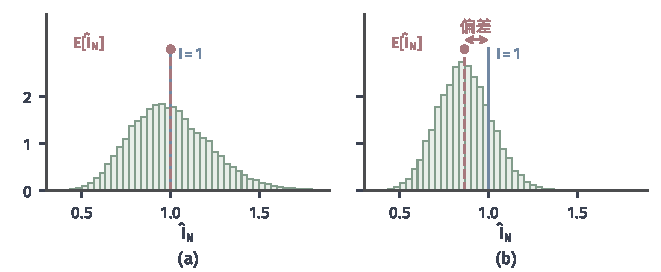
\includegraphics[width=112mm]{figures/07-probability/08-sampling-and-integration/matplotlib/mcerr-bias-spread/figure.pdf}
 \caption{估计$\mathbb{E}[X]$，$X\sim\operatorname{Exp}(1)$，每次用$N=20$个样本，重复$20000$次（种子$3101$）。绿色直方图为$\hat{I}_N$的分布，蓝线为$I=1$，红色虚线与红点为$\hat{I}_N$的平均。(a)精确的逆分位数程序；(b)把输出截到$2$的程序，红色箭头为偏差$-\mathrm{e}^{-2}$。}
 \label{fig:mcerr-bias-spread}
\end{BookInlineFigure}


\section{独立样本的误差}
\label{sec:mcerr-iid}

最理想的情形是生成程序给出独立且精确服从$\pi$的样本$X_1,\dots,X_N$。这时偏差为零：由上一节，每个$X_i$都服从$\pi$，所以$\mathbb{E}[\hat{I}_N]=I$。$f(X_1),f(X_2),\dots$独立同分布且可积，由第~\ref{chap:laws-of-large-numbers}章的强大数律，
\begin{equation}
 \hat{I}_N\xrightarrow{\mathrm{a.s.}}I .
 \label{eq:mcerr-consistency}
\end{equation}
无偏说的是平均意义下没有系统偏离，一致性说的是几乎每一次计算都会随$N$增大而接近$I$。两者都不回答一个实际问题：给定的$N$下误差有多大，或者要达到给定精度需要多大的$N$。回答它需要比可积更多的信息，所需的矩条件也决定了能给出什么样的保证。

\subsection{有限样本误差界}
\label{sec:mcerr-finite-bound}

第一种保证对每个具体的$N$成立，代价是要求$f$的二阶矩有限。记$\sigma_f^{2}=\operatorname{Var}_{\pi}(f)$，即$f(X)$在$X\sim\pi$时的方差。

\begin{theorem}[独立样本平均的误差界]
\label{thm:mcerr-iid-bound}
设$X_1,\dots,X_N$独立且都服从$\pi$，$\mathbb{E}_{\pi}[f^{2}]<\infty$。则
\begin{equation}
 \operatorname{Var}(\hat{I}_N)=\frac{\sigma_f^{2}}{N},\qquad \sqrt{\mathbb{E}\bigl[(\hat{I}_N-I)^{2}\bigr]}=\frac{\sigma_f}{\sqrt{N}} ,
 \label{eq:mcerr-iid-var}
\end{equation}
并且对每个$\varepsilon>0$，
\begin{equation}
 \mathbb{P}\bigl(\lvert\hat{I}_N-I\rvert\geq\varepsilon\bigr)\leq\frac{\sigma_f^{2}}{N\varepsilon^{2}} .
 \label{eq:mcerr-chebyshev}
\end{equation}
\end{theorem}

\begin{proof}
独立随机变量和的方差等于方差之和，所以
\[
 \operatorname{Var}(\hat{I}_N)=\frac{1}{N^{2}}\sum_{i=1}^{N}\operatorname{Var}\bigl(f(X_i)\bigr)=\frac{N\sigma_f^{2}}{N^{2}}=\frac{\sigma_f^{2}}{N} .
\]
偏差为零，由定理~\ref{thm:mcerr-mse}，均方误差等于这个方差，开方得到均方根误差。对$\hat{I}_N$用第~\ref{chap:tail-probabilities}章的Chebyshev不等式，就得到式~\eqref{eq:mcerr-chebyshev}。
\end{proof}

式~\eqref{eq:mcerr-iid-var}是Monte Carlo方法最重要的一个公式。误差按$N^{-1/2}$缩小，与$\mathcal{X}$的维数没有直接关系；维数只通过$\sigma_f$间接进入。精度提高到十倍，样本数要增加到一百倍。反过来解式~\eqref{eq:mcerr-chebyshev}：要使误差超过$\varepsilon$的概率不超过$\delta$，只需
\begin{equation}
 N\geq\frac{\sigma_f^{2}}{\delta\varepsilon^{2}} .
 \label{eq:mcerr-sample-size}
\end{equation}

\paragraph{算一个具体的样本量}
对$f(u)=\mathrm{e}^{u}$，$\pi=\operatorname{Unif}(0,1)$，先求二阶矩
\[
 \mathbb{E}[\mathrm{e}^{2U}]=\int_0^1\mathrm{e}^{2u}\,\mathrm{d}u=\frac{\mathrm{e}^{2}-1}{2}=3.1945 .
\]
再减去$I^{2}=(\mathrm{e}-1)^{2}=2.9525$，得到
\[
 \sigma_f^{2}=3.1945-2.9525=0.2420,\qquad \sigma_f=0.4920 .
\]
$N=100$时均方根误差为$0.0492$，$N=10^{4}$时为$0.00492$。图~\ref{fig:mcerr-rmse-rate}(a)把每个$N$下$1000$次独立重复得到的均方根误差与$\sigma_f/\sqrt{N}$画在双对数坐标中，点落在斜率为$-1/2$的直线上。

取$\varepsilon=0.01$，$\delta=0.05$，式~\eqref{eq:mcerr-sample-size}给出
\[
 N\geq\frac{0.2420}{0.05\times10^{-4}}=48407.1 ,
\]
即$N=48408$足够。图~\ref{fig:mcerr-chebyshev}比较了这个上界与实际概率。实际概率在$N=10^{4}$时已经降到约$0.044$；下一小节的正态近似给出所需样本量约$9298$。Chebyshev界保守了大约五倍，但它对每个$N$、对所有方差为$0.2420$的被积函数都成立，不需要任何极限论证。若$f$有界，第~\ref{chap:tail-probabilities}章的指数矩方法还能把对$\delta$的依赖从$1/\delta$改进为$\ln(1/\delta)$。

\begin{BookInlineFigure}
 \centering
 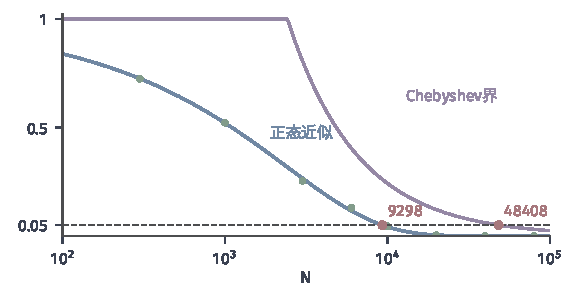
\includegraphics[width=96mm]{figures/07-probability/08-sampling-and-integration/matplotlib/mcerr-chebyshev/figure.pdf}
 \caption{$f(u)=\mathrm{e}^{u}$的样本平均误差至少为$\varepsilon=0.01$的概率。紫线为Chebyshev界$\min\{1,\sigma_f^{2}/(N\varepsilon^{2})\}$，蓝线为正态近似$2(1-\Phi(\varepsilon\sqrt{N}/\sigma_f))$，绿点为每个$N$下$2000$次重复的频率（种子$3104$）。红点标出两条曲线降到$0.05$时的样本量。}
 \label{fig:mcerr-chebyshev}
\end{BookInlineFigure}

\paragraph{二阶矩不可省}
$N^{-1/2}$的尺度完全来自方差有限。只有$\mathbb{E}_{\pi}\lvert f\rvert<\infty$时，式~\eqref{eq:mcerr-consistency}仍然成立，但误差缩小的速度可以慢得多。取$f(u)=u^{-3/4}$，$\pi=\operatorname{Unif}(0,1)$，则
\[
 I=\int_0^1u^{-3/4}\,\mathrm{d}u=4,\qquad \mathbb{E}[f(U)^{2}]=\int_0^1u^{-3/2}\,\mathrm{d}u=\infty .
\]
$f$在$0$附近趋于无穷，偶尔抽到很小的$u$，就产生一个很大的函数值。

这些大值决定了误差的尺度。$f(U)>t$当且仅当$U<t^{-4/3}$，所以
\[
 \mathbb{P}\bigl(f(U)>t\bigr)=t^{-4/3},\qquad t\geq1 .
\]
$N$个样本中至少有一个超过$t$的概率约为$Nt^{-4/3}$，它在$t\approx N^{3/4}$时变为一的量级。于是$N$个样本中最大的函数值通常在$N^{3/4}$附近，它对平均的贡献约为$N^{3/4}/N=N^{-1/4}$。每个尺度上都以不可忽略的概率出现这样的大项，平均的误差也就按$N^{-1/4}$而不是$N^{-1/2}$缩小。把这个论证写严格，需要独立和在无穷方差下的极限理论，篇幅较长，读者可查阅~\scite{math-kallenberg2021probability}。

图~\ref{fig:mcerr-heavy-paths}(a)是五次运行的运行平均：路径大部分时间偏低，每遇到一个很小的$u$就向上跳一次，然后慢慢回落。图(b)画出最大单项对平均的贡献$\max_{i\leq N}f(U_i)/N$，它沿着$N^{-1/4}$下降。图~\ref{fig:mcerr-rmse-rate}(b)用中位绝对误差衡量精度（均方误差在这里是无穷），它从$N=100$时的$0.986$降到$N=10^{5}$时的$0.172$，比值$5.73$与$1000^{1/4}=5.62$相符。按这个速度，误差缩小到十分之一要把样本数增加一万倍。

\begin{BookInlineFigure}
 \centering
 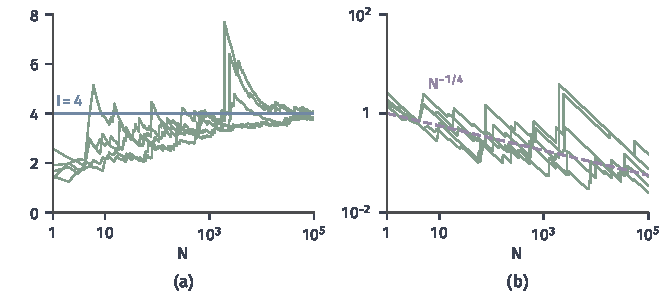
\includegraphics[width=112mm]{figures/07-probability/08-sampling-and-integration/matplotlib/mcerr-heavy-paths/figure.pdf}
 \caption{$f(u)=u^{-3/4}$的五次独立运行（种子$3105$至$3109$），横轴为对数刻度。(a)运行平均（绿线）与$I=4$（蓝线）；(b)最大单项的贡献$\max_{i\leq N}f(U_i)/N$（绿线）与参考线$N^{-1/4}$（紫色虚线），纵轴为对数刻度。}
 \label{fig:mcerr-heavy-paths}
\end{BookInlineFigure}

\begin{BookInlineFigure}
 \centering
 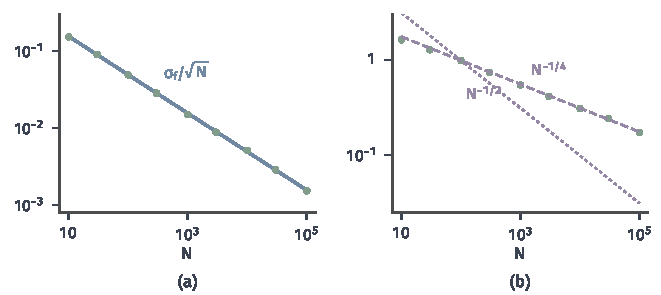
\includegraphics[width=112mm]{figures/07-probability/08-sampling-and-integration/matplotlib/mcerr-rmse-rate/figure.pdf}
 \caption{误差随样本数的变化，双对数坐标，每个$N$重复$1000$次。(a)$f(u)=\mathrm{e}^{u}$：绿点为模拟的均方根误差（种子$3102$），蓝线为$\sigma_f/\sqrt{N}$；(b)$f(u)=u^{-3/4}$：绿点为中位绝对误差（种子$3103$），紫色虚线与点线分别是斜率$-1/4$与$-1/2$的参考线。}
 \label{fig:mcerr-rmse-rate}
\end{BookInlineFigure}

\subsection{渐近误差区间}
\label{sec:mcerr-asymptotic-interval}

Chebyshev界保守，因为它只用了方差。样本数较大时，中心极限定理给出误差的近似分布，从而给出更紧的误差范围。实际计算中$\sigma_f$通常未知，要用同一批样本估计它。样本函数值的样本方差记为
\begin{equation}
 S_N^{2}=\frac{1}{N-1}\sum_{i=1}^{N}\bigl(f(X_i)-\hat{I}_N\bigr)^{2},\qquad N\geq2 .
 \label{eq:mcerr-sample-var}
\end{equation}

\begin{theorem}[独立样本的渐近误差区间]
\label{thm:mcerr-iid-clt}
设$X_1,X_2,\dots$独立且都服从$\pi$，$0<\sigma_f^{2}<\infty$。则
\begin{equation}
 \frac{\sqrt{N}\,(\hat{I}_N-I)}{S_N}\xrightarrow{\mathrm{d}}\mathcal{N}(0,1) .
 \label{eq:mcerr-studentized}
\end{equation}
因此对$0<\alpha<1$及$z=\Phi^{-1}(1-\alpha/2)$，
\begin{equation}
 \lim_{N\to\infty}\mathbb{P}\Bigl(I\in\Bigl[\hat{I}_N-\frac{zS_N}{\sqrt{N}},\ \hat{I}_N+\frac{zS_N}{\sqrt{N}}\Bigr]\Bigr)=1-\alpha .
 \label{eq:mcerr-iid-interval}
\end{equation}
\end{theorem}

\begin{proof}
$f(X_i)$独立同分布，方差为有限正数$\sigma_f^{2}$。由第~\ref{chap:central-limit-theorem}章独立同分布的中心极限定理，
\[
 \frac{\sqrt{N}\,(\hat{I}_N-I)}{\sigma_f}\xrightarrow{\mathrm{d}}\mathcal{N}(0,1) .
\]
由第~\ref{chap:laws-of-large-numbers}章样本方差的强大数律，$S_N^{2}\to\sigma_f^{2}$几乎必然成立，因而$\sigma_f/S_N\to1$依概率成立（$S_N=0$的概率趋于零，在该事件上任意规定比值即可）。式~\eqref{eq:mcerr-studentized}的左边是上式左边乘以$\sigma_f/S_N$，由第~\ref{chap:weak-convergence-of-distributions}章的Slutsky定理，乘积依分布收敛到$\mathcal{N}(0,1)$。

标准正态分布函数连续，由同一章的分布函数判据，对每个$z$，
\[
 \mathbb{P}\Bigl(\Bigl\lvert\frac{\sqrt{N}(\hat{I}_N-I)}{S_N}\Bigr\rvert\leq z\Bigr)\to\Phi(z)-\Phi(-z)=1-\alpha .
\]
左边的事件正是$I$落在式~\eqref{eq:mcerr-iid-interval}的区间中。
\end{proof}

式~\eqref{eq:mcerr-iid-interval}中的区间称为\term{渐近误差区间}（asymptotic error interval），$1-\alpha$称为名义覆盖概率；$\alpha=0.05$时$z=1.96$。区间宽度与$S_N/\sqrt{N}$成正比，后者称为估计的标准误差。它与Chebyshev界的区别在于保证的类型：Chebyshev界对每个$N$成立但偏松，渐近区间只在$N\to\infty$时给出正确的覆盖概率，对固定的$N$没有任何保证。若$\sigma_f$已知且三阶矩有限，第~\ref{chap:central-limit-theorem}章的Berry--Esseen界给出正态近似误差按$N^{-1/2}$缩小的上界；改用$S_N$以后还要加上方差估计的误差。

\paragraph{五个点的区间}
用上一节的五个均匀随机数。函数值的平均为$1.8233$，由式~\eqref{eq:mcerr-sample-var}，
\[
 S_5^{2}=0.3391,\qquad S_5=0.5823 .
\]
$\alpha=0.05$时区间半宽为
\[
 \frac{1.96\times0.5823}{\sqrt5}=0.5104 ,
\]
区间为$[1.3129,\,2.3337]$，包含$I=1.7183$。但这一次包含不说明区间可靠。图~\ref{fig:mcerr-rare-coverage}(b)的蓝线是每个$N$下$20000$次重复的实际覆盖频率：$N=5$时只有$0.868$，$N=20$时为$0.935$，$N\geq100$以后才与$0.95$相差无几。

\paragraph{稀有的大贡献}
覆盖概率接近名义值所需的样本数可以大得多。设$\pi=\operatorname{Unif}(0,1)$，
\[
 f(u)=1+1000\cdot\mathbf{1}_{\{u>0.999\}} .
\]
它有界，各阶矩都有限，定理~\ref{thm:mcerr-iid-clt}的条件全部满足。积分与方差分别是
\[
 I=1+1000\times0.001=2,\qquad \sigma_f^{2}=1000^{2}\times0.001\times0.999=999 .
\]
积分的一半来自一个概率只有千分之一的区域。

取$N=500$。一次也没有抽到$u>0.999$的概率是
\[
 0.999^{500}=\mathrm{e}^{500\ln0.999}=0.6064 .
\]
在这个事件上，所有函数值都等于$1$，于是$\hat{I}_N=1$，$S_N=0$，区间退化为单点$\{1\}$，不包含$I=2$。计算者看到的是一组完全一致的函数值和零标准误差，没有任何迹象显示有问题。

若恰好抽到一次，$\hat{I}_N=1+1000/500=3$。$499$个值与平均相差$-2$，一个值相差$998$，所以
\[
 S_N^{2}=\frac{499\times4+998^{2}}{499}=\frac{998000}{499}=2000 ,
\]
区间半宽为$1.96\sqrt{2000/500}=3.92$，区间$[-0.92,\,6.92]$包含$2$。把抽中次数服从$\operatorname{Bin}(500,0.001)$的各种情形逐一相加，$N=500$时的实际覆盖概率只有$0.393$。

图~\ref{fig:mcerr-rare-coverage}(b)的黄线是这个覆盖概率随$N$的变化，按二项分布精确求和得到。$N=10^{3}$时为$0.632$，$N=10^{4}$时才到$0.926$。图(a)是五次运行的运行平均：每条路径都先平稳地停在$1$，直到第一次抽中才突然跳起。在跳起之前，运行平均、样本方差和区间都“看起来稳定”。

即使把同一计算独立重复五次，五次都没有抽中的概率仍有$0.6064^{5}=0.082$。重复运行可以发现运行之间的分歧，但发现不了每次运行都漏掉的东西。定理~\ref{thm:mcerr-iid-clt}在这里并没有失效，它只说$N$足够大时覆盖概率接近名义值；“足够大”要比$1/0.001$大很多，而这个尺度是由$f$的结构决定的，从样本中看不出来。能防止这类错误的，是对$f$与$\pi$本身的分析，例如知道函数值的上界或贡献集中的区域，第~\ref{chap:variance-reduction}章的重要性采样正是利用这类信息。

\begin{BookInlineFigure}
 \centering
 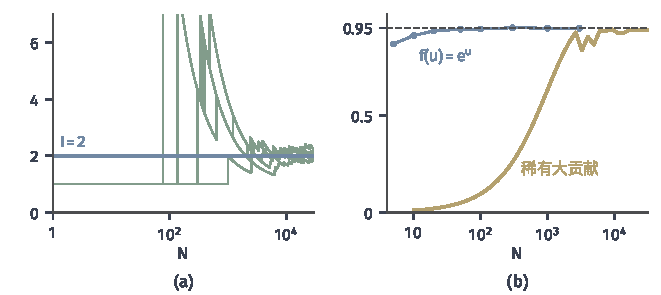
\includegraphics[width=112mm]{figures/07-probability/08-sampling-and-integration/matplotlib/mcerr-rare-coverage/figure.pdf}
 \caption{稀有大贡献$f(u)=1+1000\cdot\mathbf{1}_{\{u>0.999\}}$，$I=2$。(a)五次独立运行的运行平均（绿线，种子$3110$至$3114$）与$I$（蓝线），横轴为对数刻度；(b)渐近区间$\hat{I}_N\pm1.96S_N/\sqrt{N}$的实际覆盖概率：黄线为稀有大贡献的精确值，蓝线为$f(u)=\mathrm{e}^{u}$在每个$N$下$20000$次重复的频率（种子$3115$），虚线为名义值$0.95$。}
 \label{fig:mcerr-rare-coverage}
\end{BookInlineFigure}


\section{近似生成的偏差}
\label{sec:mcerr-approx}

实际程序很少精确地服从$\pi$。分位数没有解析式时要数值反演，连续时间的动态要离散化，有时还会像上一节的例子那样为了数值安全截断输出。设程序独立地产生服从$\tilde{\pi}$的样本，$\tilde{\pi}$与$\pi$接近但不相等。对在两种分布下都可积的$f$，记
\begin{equation}
 b=\mathbb{E}_{\tilde{\pi}}[f]-\mathbb{E}_{\pi}[f] .
 \label{eq:mcerr-approx-bias}
\end{equation}
这是由生成规律本身带来的积分偏差，与样本数无关。

\paragraph{偏差不随样本数消失}
样本独立且都服从$\tilde{\pi}$，第~\ref{sec:mcerr-iid}节的结论对$\tilde{\pi}$成立：$\hat{I}_N$几乎必然收敛到$\mathbb{E}_{\tilde{\pi}}[f]=I+b$，而不是$I$。若$\mathbb{E}_{\tilde{\pi}}[f^{2}]<\infty$，由定理~\ref{thm:mcerr-mse}，
\begin{equation}
 \mathbb{E}\bigl[(\hat{I}_N-I)^{2}\bigr]=b^{2}+\frac{\operatorname{Var}_{\tilde{\pi}}(f)}{N}\geq b^{2} .
 \label{eq:mcerr-approx-mse}
\end{equation}
增加同一近似方法的样本数只能压低第二项，均方误差最终停在$b^{2}$。

回到截断程序$\tilde{X}=\min\{X,2\}$。它的二阶矩可以由尾概率算出：
\[
 \mathbb{E}[\min\{X,T\}^{2}]=\int_0^{T}2t\,\mathrm{e}^{-t}\,\mathrm{d}t=2\bigl(1-(1+T)\mathrm{e}^{-T}\bigr) .
\]
$T=2$时它等于$1.1880$，减去均值的平方$0.8647^{2}=0.7476$，得到
\[
 \operatorname{Var}_{\tilde{\pi}}(f)=0.4403,\qquad b^{2}=\mathrm{e}^{-4}=0.0183 .
\]
两项在$N=0.4403/0.0183\approx24$时相等。样本数超过几十以后，误差几乎全由偏差决定。

图~\ref{fig:mcerr-approx-bias}(a)中五条运行平均都收敛到$1-\mathrm{e}^{-2}$，离$I=1$始终差$0.135$。图(b)比较两个程序的均方根误差：精确程序沿$1/\sqrt{N}$一直下降，截断程序在$N$超过几十后变平，停在$\lvert b\rvert$。这时只看运行平均是否稳定、标准误差是否很小，会得到一个精确地错了的答案。

\begin{BookInlineFigure}
 \centering
 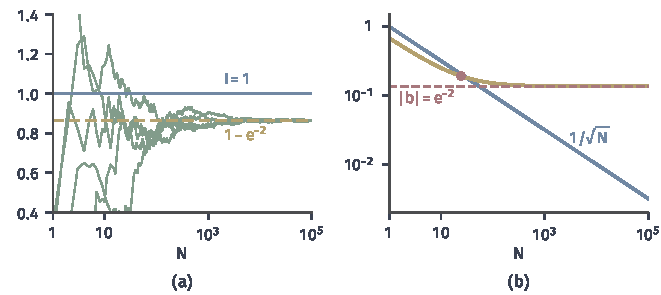
\includegraphics[width=112mm]{figures/07-probability/08-sampling-and-integration/matplotlib/mcerr-approx-bias/figure.pdf}
 \caption{截断程序$\min\{X,2\}$估计$\mathbb{E}[X]=1$，$X\sim\operatorname{Exp}(1)$，横轴为对数刻度。(a)五次运行的运行平均（绿线，种子$3116$至$3120$），蓝线为$I=1$，黄色虚线为$\tilde{\pi}$下的均值$1-\mathrm{e}^{-2}$；(b)均方根误差的精确值：蓝线为精确程序的$1/\sqrt{N}$，黄线为截断程序的$\sqrt{b^{2}+0.4403/N}$，红色虚线为$\lvert b\rvert=\mathrm{e}^{-2}$，红点标出方差项等于$b^{2}$的$N\approx24$。}
 \label{fig:mcerr-approx-bias}
\end{BookInlineFigure}

\paragraph{有界被积函数}
偏差无法从样本中读出，只能从$\tilde{\pi}$与$\pi$的差别估计出来。第~\ref{chap:distribution-comparison}章的总变差正好衡量这种差别：对有界的$f$，记$\operatorname{osc}(f)=\sup f-\inf f$，那里证明了
\begin{equation}
 \lvert b\rvert=\bigl\lvert\mathbb{E}_{\tilde{\pi}}[f]-\mathbb{E}_{\pi}[f]\bigr\rvert\leq\operatorname{osc}(f)\,d_{\mathrm{TV}}(\tilde{\pi},\pi)\leq2\sup\lvert f\rvert\,d_{\mathrm{TV}}(\tilde{\pi},\pi) .
 \label{eq:mcerr-tv-bound}
\end{equation}
所以只要知道近似分布与目标的总变差，就同时控制了所有有界被积函数的偏差。

截断程序的总变差可以直接算出。$\tilde{\pi}$在$[0,2)$上与$\pi$有相同的密度，把$\pi$在$(2,\infty)$上的质量$\mathrm{e}^{-2}$全部堆到点$2$上，如图~\ref{fig:mcerr-tv-bias}(a)。对任一事件$A$，差别只来自$A$与$\{2\}$、$(2,\infty)$的交，所以
\[
 \lvert\tilde{\pi}(A)-\pi(A)\rvert\leq\mathrm{e}^{-2},
\]
取$A=(2,\infty)$时等号成立，所以
\[
 d_{\mathrm{TV}}(\tilde{\pi},\pi)=\mathrm{e}^{-2} .
\]
对$f=\mathbf{1}_{\{x>2\}}$，$\operatorname{osc}(f)=1$，偏差恰为$-\mathrm{e}^{-2}$，式~\eqref{eq:mcerr-tv-bound}取到等号；对$f=\mathbf{1}_{\{x>1\}}$，截断不改变事件$\{X>1\}$，偏差为零。

\paragraph{无界被积函数}
对无界的$f$，总变差小并不能保证偏差小。设$\varepsilon\in(0,1)$，$c>1$，令近似分布为
\[
 \tilde{\pi}_{\varepsilon}=(1-\varepsilon)\,\pi+\varepsilon\,\delta_{c},\qquad \pi=\operatorname{Exp}(1) ,
\]
即以概率$1-\varepsilon$正常生成，以概率$\varepsilon$输出一个远处的值$c$。对任一事件$A$，
\[
 \lvert\tilde{\pi}_{\varepsilon}(A)-\pi(A)\rvert=\varepsilon\,\lvert\delta_{c}(A)-\pi(A)\rvert\leq\varepsilon ,
\]
所以$d_{\mathrm{TV}}\leq\varepsilon$。对$f(x)=x$，偏差却是$\varepsilon(c-1)$。取$c=1/\varepsilon^{2}$，总变差趋于零时偏差$1/\varepsilon-\varepsilon$趋于无穷。

图~\ref{fig:mcerr-tv-bias}(b)对照了这两种情形：有界的$f$的偏差随$\varepsilon$线性缩小，$f(x)=x$的偏差反而增大。问题出在少量质量被放到了很远的地方。总变差只问“同一事件的概率差多少”，不问质量移到了哪里；无界函数却对远处的质量非常敏感。

\begin{BookInlineFigure}
 \centering
 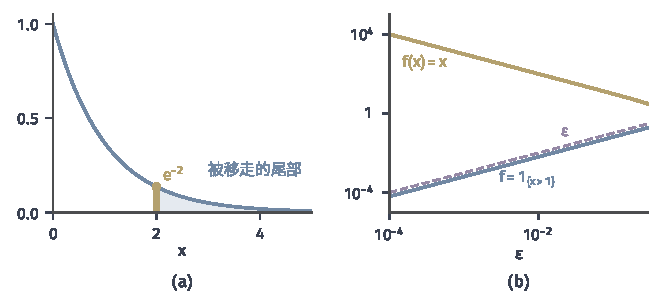
\includegraphics[width=112mm]{figures/07-probability/08-sampling-and-integration/matplotlib/mcerr-tv-bias/figure.pdf}
 \caption{总变差与积分偏差。(a)$\operatorname{Exp}(1)$的密度（蓝线）；截断程序把浅蓝区域中的尾部质量移到点$2$，形成质量为$\mathrm{e}^{-2}$的原子（黄色竖线，高度表示质量）。(b)近似分布$(1-\varepsilon)\operatorname{Exp}(1)+\varepsilon\delta_{1/\varepsilon^{2}}$的总变差不超过$\varepsilon$（紫色虚线）；蓝线为$f=\mathbf{1}_{\{x>1\}}$的偏差$\varepsilon(1-\mathrm{e}^{-1})$，黄线为$f(x)=x$的偏差$1/\varepsilon-\varepsilon$，双对数坐标。}
 \label{fig:mcerr-tv-bias}
\end{BookInlineFigure}

要让总变差重新起作用，需要控制两种分布在远处的质量。下面用二阶矩给出一个简单的结论。

\begin{lemma}[矩控制下的偏差界]
\label{lem:mcerr-moment-tv}
设$\mathbb{E}_{\pi}[f^{2}]\leq m$，$\mathbb{E}_{\tilde{\pi}}[f^{2}]\leq m$，记$d=d_{\mathrm{TV}}(\tilde{\pi},\pi)$。则
\begin{equation}
 \bigl\lvert\mathbb{E}_{\tilde{\pi}}[f]-\mathbb{E}_{\pi}[f]\bigr\rvert\leq4\sqrt{m\,d} .
 \label{eq:mcerr-moment-tv}
\end{equation}
\end{lemma}

\begin{proof}
$d=0$时两分布相同，结论成立。设$d>0$，固定截断水平$t>0$，把$f$分成有界部分与尾部：
\[
 f=f\,\mathbf{1}_{\{\lvert f\rvert\leq t\}}+f\,\mathbf{1}_{\{\lvert f\rvert>t\}} .
\]
有界部分的振幅不超过$2t$，由式~\eqref{eq:mcerr-tv-bound}，它在两分布下的期望差不超过$2td$。

尾部在$\lvert f\rvert>t$时满足$\lvert f\rvert\leq f^{2}/t$，所以对$\pi$与$\tilde{\pi}$都有
\[
 \bigl\lvert\mathbb{E}\bigl[f\,\mathbf{1}_{\{\lvert f\rvert>t\}}\bigr]\bigr\rvert\leq\frac{\mathbb{E}[f^{2}]}{t}\leq\frac{m}{t} .
\]
两分布下的尾部期望之差不超过$2m/t$。合起来，偏差不超过$2td+2m/t$。取$t=\sqrt{m/d}$，两项都等于$2\sqrt{md}$。
\end{proof}

证明里的截断水平体现了两种误差的折中：$t$越大，有界部分越宽，总变差的作用被放大；$t$越小，留在尾部的质量越多。界$4\sqrt{md}$随$d$按平方根缩小，比有界情形的线性缩小慢，这是为控制尾部付出的代价。对截断程序，$f(x)=x$在两分布下的二阶矩分别是$2$和$1.188$，取$m=2$，界为
\[
 4\sqrt{2\times0.1353}=2.081 ,
\]
远大于实际的$0.1353$，但它不依赖任何具体计算。对$\tilde{\pi}_{\varepsilon}$，二阶矩至少为$\varepsilon c^{2}=\varepsilon^{-3}$，代入后界的量级是$4/\varepsilon$，与实际偏差的量级一致：矩条件正好抓住了远处质量的作用。

\paragraph{近似转移}
用Markov链采样时，近似发生在转移这一步：理论上的转移核$K$以$\pi$为不变分布，实际程序执行的却是另一个核$\tilde{K}$。这时要先回答一个更基本的问题：$\tilde{K}$有没有不变分布，有的话它离$\pi$多远。链跑得再久，平均也只能趋向$\tilde{K}$自己的长期规律。

看一个可以算到底的例子。目标是$\pi=\mathcal{N}(0,1)$，某个由连续时间动态离散化得到的更新为
\[
 X^{(t+1)}=(1-h)X^{(t)}+\sqrt{2h}\,\xi^{(t+1)} ,
\]
其中$\xi^{(1)},\xi^{(2)},\dots$独立且服从$\mathcal{N}(0,1)$，与$X^{(0)}$独立，$h>0$是步长。若$X^{(t)}\sim\mathcal{N}(0,v)$，则$X^{(t+1)}\sim\mathcal{N}(0,(1-h)^{2}v+2h)$。令两者相等，
\[
 v=(1-h)^{2}v+2h,\qquad v=\frac{2h}{1-(1-h)^{2}}=\frac{2}{2-h},\qquad 0<h<2 .
\]
所以$0<h<2$时，$\mathcal{N}(0,2/(2-h))$是这个近似转移的不变分布，而$\pi$不是。

从任意$x$出发，展开递推得到
\[
 X^{(t)}=(1-h)^{t}x+\sum_{j=1}^{t}(1-h)^{t-j}\sqrt{2h}\,\xi^{(j)} ,
\]
它服从均值为$(1-h)^{t}x$、方差为$2h\sum_{j<t}(1-h)^{2j}$的高斯分布。$\lvert1-h\rvert<1$时，均值趋于零，方差趋于$v$，链确实趋向这个不变分布。取$h=0.5$，$v=4/3$。对$f(x)=x^{2}$，偏差为$4/3-1=1/3$；对有界的$f=\mathbf{1}_{\{\lvert x\rvert\leq1\}}$，
\[
 \mathbb{P}_{\mathcal{N}(0,4/3)}\bigl(\lvert X\rvert\leq1\bigr)=2\Phi\bigl(\sqrt{3}/2\bigr)-1=0.6135 ,
\]
而目标值是$2\Phi(1)-1=0.6827$，偏差为$-0.0692$。图~\ref{fig:mcerr-approx-chain}(b)中，$10^{5}$步的直方图贴合的是$\mathcal{N}(0,4/3)$，不是$\pi$。

$h\geq2$时，不变分布根本不存在。设$\mu$是不变分布，$\phi$是它的特征函数，则$X\sim\mu$与独立的$\xi$满足$(1-h)X+\sqrt{2h}\,\xi\sim\mu$，即
\[
 \phi(s)=\phi\bigl((1-h)s\bigr)\,\mathrm{e}^{-hs^{2}} .
\]
记$c=\lvert1-h\rvert\geq1$。特征函数的模不超过$1$，把上式反复代入$k$次，
\[
 \lvert\phi(s)\rvert\leq\exp\Bigl(-hs^{2}\sum_{j=0}^{k-1}c^{2j}\Bigr)\leq\mathrm{e}^{-khs^{2}} .
\]
令$k\to\infty$，对每个$s\neq0$得$\phi(s)=0$。这与特征函数在$0$处连续且$\phi(0)=1$矛盾。图~\ref{fig:mcerr-approx-chain}(a)画出不变方差$2/(2-h)$，它在$h\to2$时趋于无穷。

\begin{BookInlineFigure}
 \centering
 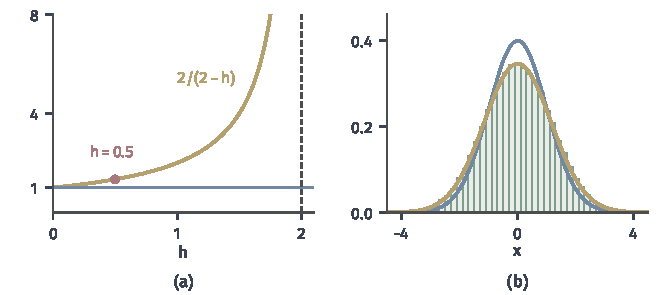
\includegraphics[width=112mm]{figures/07-probability/08-sampling-and-integration/matplotlib/mcerr-approx-chain/figure.pdf}
 \caption{近似转移$X'=(1-h)X+\sqrt{2h}\,\xi$，目标为$\mathcal{N}(0,1)$。(a)不变分布的方差$2/(2-h)$（黄线）与目标方差$1$（蓝线），灰色虚线为$h=2$，红点为$h=0.5$；(b)$h=0.5$时从$0$出发运行$10^{5}$步的直方图（绿色，种子$3121$），蓝线为目标密度，黄线为不变分布$\mathcal{N}(0,4/3)$的密度。}
 \label{fig:mcerr-approx-chain}
\end{BookInlineFigure}

这个例子显示了近似链需要分两步检查。先确认近似转移存在不变分布、并且链会趋向它；再估计它与$\pi$的差，必要时减小步长或用第~\ref{chap:sample-generation}章的Metropolis接受步骤校正，使$\pi$恢复为精确的不变分布。两步都与运行长度无关。


\section{链初值的影响}
\label{sec:mcerr-initial}

现在设转移是精确的。第~\ref{chap:sample-generation}章用转移核$K(x,A)$描述链：当前状态为$x$时，下一状态落入$A$的概率为$K(x,A)$。若
\[
 \int_{\mathcal{X}}K(x,A)\,\pi(\mathrm{d}x)=\pi(A)\qquad\text{对每个事件}A ,
\]
就称$\pi$是不变分布。链从$X^{(0)}$出发，依次生成$X^{(1)},X^{(2)},\dots$，用
\begin{equation}
 \hat{I}_N=\frac1N\sum_{t=1}^{N}f\bigl(X^{(t)}\bigr)
 \label{eq:mcerr-chain-average}
\end{equation}
估计$I$。这一节研究链从哪里出发怎样影响这个平均的偏差。

\paragraph{从目标分布出发}
若$X^{(0)}\sim\pi$，由不变性，$X^{(1)}$的分布是
\[
 \mathbb{P}(X^{(1)}\in A)=\int K(x,A)\,\pi(\mathrm{d}x)=\pi(A) ,
\]
依次类推，每个$X^{(t)}$都服从$\pi$。由第~\ref{sec:mcerr-estimator}节，偏差只看各项的分布，所以$\hat{I}_N$无偏，尽管各项高度相关。这样的链称为平稳的：任意时刻的状态都服从$\pi$。

\paragraph{从一般初值出发}
实际中能精确从$\pi$出发，往往就不需要链了。设$X^{(0)}\sim\mu$。记$K^{t}(x,\cdot)$为从$x$出发$t$步后状态的分布，则$X^{(t)}$的分布是$\mu K^{t}=\int\mu(\mathrm{d}x)\,K^{t}(x,\cdot)$，一般不等于$\pi$。设各项可积，偏差为
\begin{equation}
 b_N=\frac1N\sum_{t=1}^{N}\Bigl(\mathbb{E}_{\mu K^{t}}[f]-I\Bigr) .
 \label{eq:mcerr-initial-bias}
\end{equation}
偏差的大小取决于边缘分布$\mu K^{t}$趋近$\pi$的快慢。

\paragraph{一条可以算到底的链}
下面这条链贯穿本章后半部分。取$\pi=\mathcal{N}(0,1)$，$\lvert\rho\rvert<1$，令
\begin{equation}
 X^{(t+1)}=\rho X^{(t)}+\sqrt{1-\rho^{2}}\,\xi^{(t+1)} ,
 \label{eq:mcerr-ar1}
\end{equation}
其中$\xi^{(t)}$独立且服从$\mathcal{N}(0,1)$，与$X^{(0)}$独立。若$X^{(t)}\sim\mathcal{N}(0,1)$，则$X^{(t+1)}$服从均值为$0$、方差为$\rho^{2}+(1-\rho^{2})=1$的高斯分布，所以$\pi$是不变分布。$\rho$越接近$1$，每步保留的旧状态越多，链移动越慢。

从$X^{(0)}=x_0$出发，展开递推，
\[
 X^{(t)}=\rho^{t}x_0+\sqrt{1-\rho^{2}}\sum_{j=1}^{t}\rho^{t-j}\xi^{(j)} .
\]
后一项是独立高斯变量的线性组合，方差为$(1-\rho^{2})\sum_{j=0}^{t-1}\rho^{2j}=1-\rho^{2t}$，所以
\begin{equation}
 K^{t}(x_0,\cdot)=\mathcal{N}\bigl(\rho^{t}x_0,\ 1-\rho^{2t}\bigr) .
 \label{eq:mcerr-ar1-marginal}
\end{equation}
均值以几何速度$\rho^{t}$忘掉初值。对$f(x)=x$，$I=0$，由式~\eqref{eq:mcerr-initial-bias}，偏差为几何级数之和：
\[
 b_N=\frac{x_0}{N}\sum_{t=1}^{N}\rho^{t}=\frac{x_0\,\rho\,(1-\rho^{N})}{N(1-\rho)} .
\]

取$\rho=0.9$，$x_0=10$。偏差约为$90/N$：
\[
 b_{100}=0.900,\qquad b_{1000}=0.0900 .
\]
第~\ref{sec:mcerr-long-run}小节会算出平稳时这条链平均的标准差约为$\sqrt{19/N}$，$N=100$时为$0.436$，比偏差还小。偏差按$1/N$缩小，标准差按$1/\sqrt{N}$缩小，所以记录足够长时初值的影响终将被波动淹没，但在中等长度上它可以是误差的主要部分。图~\ref{fig:mcerr-burnin}(a)是$20$条从$10$出发的路径，它们沿着$0.9^{t}\times10$向$0$靠拢，大约$40$步以后才混入平稳的波动带。

\paragraph{舍弃初始一段}
常用的办法是先运行$b$步不记录，再平均接下来的$N$个状态，被舍弃的这一段称为\term{预烧期}（burn-in period）。对上面的链，平均$X^{(b+1)},\dots,X^{(b+N)}$的偏差是
\[
 \frac{x_0\,\rho^{b+1}(1-\rho^{N})}{N(1-\rho)} .
\]
$N=100$时，$b=20$把偏差从$0.900$降到$0.109$，$b=50$降到$0.0046$，如图~\ref{fig:mcerr-burnin}(b)。

\begin{BookInlineFigure}
 \centering
 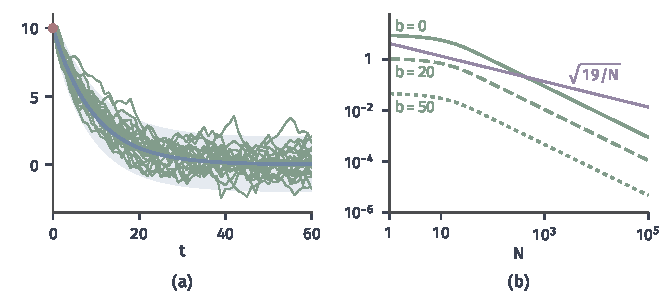
\includegraphics[width=112mm]{figures/07-probability/08-sampling-and-integration/matplotlib/mcerr-burnin/figure.pdf}
 \caption{链~\eqref{eq:mcerr-ar1}在$\rho=0.9$时从$x_0=10$（红点）出发。(a)$20$条路径（绿线，种子$3122$），蓝线为边缘均值$0.9^{t}x_0$，浅蓝带为边缘均值加减两倍边缘标准差；(b)舍弃前$b$步后平均$N$步的偏差精确值（绿色实线、虚线、点线分别为$b=0,20,50$），紫线为平稳时的标准差$\sqrt{19/N}$，双对数坐标。}
 \label{fig:mcerr-burnin}
\end{BookInlineFigure}

预烧期之所以有效，是因为这里知道边缘分布以$\rho^{t}$的速度靠近$\pi$。一般地，若对有界的$f$已知$d_{\mathrm{TV}}(\mu K^{t},\pi)\leq Cr^{t}$，$0<r<1$，由式~\eqref{eq:mcerr-tv-bound}与式~\eqref{eq:mcerr-initial-bias}，舍弃$b$步后
\begin{equation}
 \lvert b_N\rvert\leq\frac{\operatorname{osc}(f)}{N}\sum_{t=b+1}^{b+N}Cr^{t}\leq\frac{\operatorname{osc}(f)\,C\,r^{b+1}}{N(1-r)} .
 \label{eq:mcerr-burnin-bound}
\end{equation}
没有这类收敛控制，预烧期就没有依据。最极端的例子是始终停在原地的转移$K(x,\cdot)=\delta_{x}$：每个分布都是它的不变分布，但从$x_0$出发的链永远停在$x_0$，舍弃多少步都不改变$\hat{I}_N=f(x_0)$。第~\ref{sec:mcerr-diagnostics}小节还会看到更隐蔽的情形：链在一个局部区域内看起来已经平稳，却始终没有到达目标的另一部分。

即使有收敛控制，舍弃之后剩下的样本也不是精确平稳的。在式~\eqref{eq:mcerr-ar1-marginal}中，任何有限的$t$都有$1-\rho^{2t}<1$，$K^{t}(x_0,\cdot)$从来不等于$\pi$。预烧期只是把偏差压到可以忽略的量级，这个量级需要由式~\eqref{eq:mcerr-burnin-bound}这样的估计给出。

\paragraph{无界被积函数}
式~\eqref{eq:mcerr-burnin-bound}要求$f$有界。对无界的$f$，即使$\mu K^{t}$收敛到$\pi$，期望也未必收敛。第~\ref{chap:random-variable-convergence}章与第~\ref{chap:weak-convergence-of-distributions}章说明，分布收敛之外还需要$f(X^{(t)})$一致可积，才能保证$\mathbb{E}[f(X^{(t)})]\to\mathbb{E}_{\pi}[f]$。

仍用链~\eqref{eq:mcerr-ar1}，但让$X^{(0)}$服从二阶矩无穷的分布，例如标准Cauchy分布，取$f(x)=x^{2}$。$X^{(t)}=\rho^{t}X^{(0)}+G_t$，其中$G_t$是与$X^{(0)}$独立的高斯变量。给定$G_t$时，$\rho^{t}X^{(0)}+G_t$的二阶矩为无穷，所以对每个$t$，
\[
 \mathbb{E}\bigl[(X^{(t)})^{2}\bigr]=\infty .
\]
另一方面，$\rho^{t}X^{(0)}\to0$依概率成立，由Slutsky定理，$X^{(t)}$依分布收敛到$\mathcal{N}(0,1)$。于是对每个$N$和每个预烧期长度，$\mathbb{E}[\hat{I}_N]=\infty$，偏差没有意义，舍弃初始段也无济于事。初值的尾部经过任意有限步都没有被完全忘掉，正是这种残留破坏了一致可积性。


\section{相关平均的方差}
\label{sec:mcerr-correlated}

上一节处理的是链平均的偏差，现在把它放在一边，假定链从$\pi$出发，于是$\hat{I}_N$无偏，误差只剩随机波动。链的相邻状态相关，式~\eqref{eq:mcerr-iid-var}的推导用到了独立性，不能照搬。相关性究竟让波动变大还是变小，变多少？先对固定的$N$精确计算方差，再看$N$很大时它的主要部分。

\subsection{平稳平均的方差}
\label{sec:mcerr-stationary-var}

设链平稳，$\mathbb{E}_{\pi}[f^{2}]<\infty$。对任意时刻$s$，$X^{(s)}\sim\pi$，并且从$X^{(s)}$往后按同一个核演化，所以$(X^{(s)},X^{(s+k)})$与$(X^{(0)},X^{(k)})$有相同的联合分布。于是两时刻函数值的协方差只依赖时间差$k$，记
\begin{equation}
 \gamma_k=\operatorname{Cov}_{\pi}\bigl(f(X^{(0)}),f(X^{(k)})\bigr),\qquad k=0,1,2,\dots
 \label{eq:mcerr-autocov}
\end{equation}
它称为$f$沿链的\term{自协方差}（autocovariance）。$\gamma_0=\operatorname{Var}_{\pi}(f)$，由Cauchy--Schwarz不等式，$\lvert\gamma_k\rvert\leq\gamma_0$。

\begin{theorem}[平稳平均的方差]
\label{thm:mcerr-stationary-var}
设链平稳，$\mathbb{E}_{\pi}[f^{2}]<\infty$。则对每个$N\geq1$，
\begin{equation}
 \operatorname{Var}(\hat{I}_N)=\frac1N\Bigl[\gamma_0+2\sum_{k=1}^{N-1}\Bigl(1-\frac{k}{N}\Bigr)\gamma_k\Bigr] .
 \label{eq:mcerr-stationary-var}
\end{equation}
\end{theorem}

\begin{proof}
记$Y_t=f(X^{(t)})$。和的方差等于全部协方差之和，
\[
 \operatorname{Var}\Bigl(\sum_{t=1}^{N}Y_t\Bigr)=\sum_{s=1}^{N}\sum_{t=1}^{N}\operatorname{Cov}(Y_s,Y_t)=\sum_{s=1}^{N}\sum_{t=1}^{N}\gamma_{\lvert s-t\rvert} .
\]
在$N\times N$的下标方阵中，$\lvert s-t\rvert=0$的格子有$N$个（对角线）；对$1\leq k\leq N-1$，$\lvert s-t\rvert=k$的格子在对角线两侧各有$N-k$个。按$k$合并，
\[
 \operatorname{Var}\Bigl(\sum_{t=1}^{N}Y_t\Bigr)=N\gamma_0+2\sum_{k=1}^{N-1}(N-k)\gamma_k .
\]
两边除以$N^{2}$即得。
\end{proof}

与独立情形比较，式~\eqref{eq:mcerr-stationary-var}多了方括号里的求和。各$\gamma_k$为正时，方差大于$\gamma_0/N$：相邻状态差不多，第二个样本带来的新信息少于一个独立样本，好比反复询问同一户人家。各$\gamma_k$正负交替时，方差可以小于$\gamma_0/N$：相邻状态落在两侧，平均时互相抵消。所以链输出的方差既可能比独立平均大，也可能比它小；直接把$S_N^{2}/N$当作链平均的方差，没有任何依据。

\paragraph{例子中的自协方差}
对链~\eqref{eq:mcerr-ar1}与$f(x)=x$，$X^{(k)}$等于$\rho^{k}X^{(0)}$加上一个与$X^{(0)}$独立的项，所以
\[
 \gamma_k=\operatorname{Cov}\bigl(X^{(0)},\rho^{k}X^{(0)}\bigr)=\rho^{k} .
\]
对$f(x)=x^{2}$，记$Z$为与$X^{(0)}$独立的标准正态变量，$X^{(k)}=\rho^{k}X^{(0)}+\sqrt{1-\rho^{2k}}\,Z$，平方后
\[
 (X^{(k)})^{2}=\rho^{2k}(X^{(0)})^{2}+2\rho^{k}\sqrt{1-\rho^{2k}}\,X^{(0)}Z+(1-\rho^{2k})Z^{2} .
\]
与$(X^{(0)})^{2}$求协方差时，第二项的协方差是$\mathbb{E}[(X^{(0)})^{3}]\,\mathbb{E}[Z]=0$，第三项与$X^{(0)}$独立，只剩第一项。标准正态变量平方的方差是$2$，所以$\gamma_k=2\rho^{2k}$。

\paragraph{四步的平均}
取$N=4$，$f(x)=x$。$\rho=0.9$时，由式~\eqref{eq:mcerr-stationary-var}，
\[
 \operatorname{Var}(\hat{I}_4)=\frac14\bigl[1+2(0.75\times0.9+0.5\times0.81+0.25\times0.729)\bigr]=\frac{3.5245}{4}=0.8811 .
\]
$\rho=-0.5$时，
\[
 \operatorname{Var}(\hat{I}_4)=\frac14\bigl[1+2(-0.75\times0.5+0.5\times0.25-0.25\times0.125)\bigr]=\frac{0.4375}{4}=0.1094 .
\]
同样长度的独立平均方差是$0.25$。正相关的链把方差放大到约$3.5$倍，负相关的链把它缩小到约$0.44$倍。

图~\ref{fig:mcerr-ar-paths}用同一串噪声画出三条平稳链。$\rho=0.9$的路径缓慢起伏，$80$步的平均为$0.45$；$\rho=0$即独立样本，平均为$0.097$；$\rho=-0.5$的路径在$0$两侧来回跳，平均只有$0.055$。图~\ref{fig:mcerr-autocov}(a)画出两种$\rho$下的$\gamma_k$。

\begin{BookInlineFigure}
 \centering
 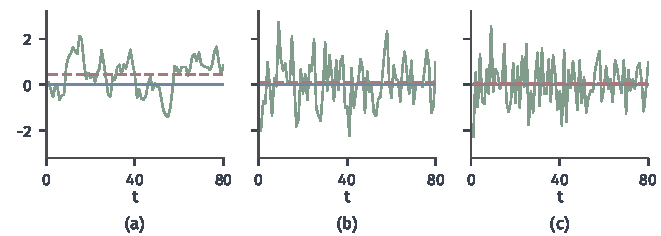
\includegraphics[width=112mm]{figures/07-probability/08-sampling-and-integration/matplotlib/mcerr-ar-paths/figure.pdf}
 \caption{平稳链~\eqref{eq:mcerr-ar1}的$80$步路径（绿线），三图使用同一串噪声与初值（种子$3129$）。(a)$\rho=0.9$；(b)$\rho=0$；(c)$\rho=-0.5$。蓝线为$I=0$，红色虚线为$80$步的平均。}
 \label{fig:mcerr-ar-paths}
\end{BookInlineFigure}

\subsection{长期方差}
\label{sec:mcerr-long-run}

链平均的方差公式~\eqref{eq:mcerr-stationary-var}含有$N$个项，比较两条链或两个被积函数时不方便。$N$很大时，权重$1-k/N$对固定的$k$趋于$1$，方括号趋于一个与$N$无关的数，它就是比较精度时需要的量。

\begin{definition}[长期方差]
\label{def:mcerr-long-run}
设链平稳，$\mathbb{E}_{\pi}[f^{2}]<\infty$，且$\sum_{k\geq1}\lvert\gamma_k\rvert<\infty$。称
\begin{equation}
 \sigma_{\mathrm{LR}}^{2}=\gamma_0+2\sum_{k=1}^{\infty}\gamma_k
 \label{eq:mcerr-long-run}
\end{equation}
为$f$沿链的\term{长期方差}（long-run variance）。
\end{definition}

\begin{theorem}[方差的极限]
\label{thm:mcerr-long-run-limit}
在定义~\ref{def:mcerr-long-run}的条件下，
\begin{equation}
 \lim_{N\to\infty}N\operatorname{Var}(\hat{I}_N)=\sigma_{\mathrm{LR}}^{2} .
 \label{eq:mcerr-nvar-limit}
\end{equation}
\end{theorem}

\begin{proof}
由式~\eqref{eq:mcerr-stationary-var}与式~\eqref{eq:mcerr-long-run}，
\[
 N\operatorname{Var}(\hat{I}_N)-\sigma_{\mathrm{LR}}^{2}=-2\sum_{k=N}^{\infty}\gamma_k-2\sum_{k=1}^{N-1}\frac{k}{N}\gamma_k .
\]
第一项是收敛级数的尾部，趋于零。第二项中第$k$项$(k/N)\gamma_k\mathbf{1}_{\{k<N\}}$的绝对值不超过$\lvert\gamma_k\rvert$，而且对固定的$k$，它随$N\to\infty$趋于零。$\lvert\gamma_k\rvert$可和，由支配收敛定理（用于计数测度上的级数），第二项也趋于零。
\end{proof}

于是$N$大时$\operatorname{Var}(\hat{I}_N)\approx\sigma_{\mathrm{LR}}^{2}/N$，链平均仍按$N^{-1/2}$收缩，只是把独立情形的$\gamma_0$换成了$\sigma_{\mathrm{LR}}^{2}$。对链~\eqref{eq:mcerr-ar1}与$f(x)=x$，
\[
 \sigma_{\mathrm{LR}}^{2}=1+2\sum_{k=1}^{\infty}\rho^{k}=1+\frac{2\rho}{1-\rho}=\frac{1+\rho}{1-\rho} .
\]
$\rho=0.9$时为$19$，$\rho=-0.5$时为$1/3$。图~\ref{fig:mcerr-autocov}(b)画出$N\operatorname{Var}(\hat{I}_N)$的精确值：$\rho=0.9$时，$N=4$为$3.52$，$N=100$为$17.20$，$N=1000$为$18.82$，逐步接近$19$。接近的快慢由$\gamma_k$衰减的快慢决定。

\begin{BookInlineFigure}
 \centering
 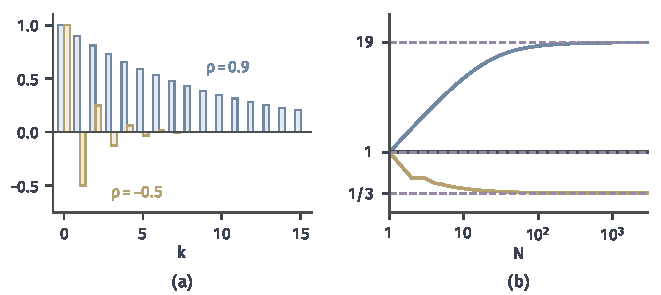
\includegraphics[width=112mm]{figures/07-probability/08-sampling-and-integration/matplotlib/mcerr-autocov/figure.pdf}
 \caption{平稳链~\eqref{eq:mcerr-ar1}与$f(x)=x$。(a)自协方差$\gamma_k=\rho^{k}$，蓝色为$\rho=0.9$，黄色为$\rho=-0.5$；(b)由式~\eqref{eq:mcerr-stationary-var}算出的$N\operatorname{Var}(\hat{I}_N)$，蓝、灰、黄线分别对应$\rho=0.9,0,-0.5$，紫色虚线为长期方差$19,1,1/3$，双对数坐标。}
 \label{fig:mcerr-autocov}
\end{BookInlineFigure}

\paragraph{可和条件不成立时}
协方差不可和时，方差的极限可以不存在。考虑状态空间$\{0,1\}$上始终停在原地的链，从$\pi=(1/2,1/2)$出发，取$f$为状态$1$的示性函数。每一步的状态都等于$X^{(0)}$，所以$\gamma_k=1/4$对所有$k$成立，级数发散；实际上$\hat{I}_N=f(X^{(0)})$，$\operatorname{Var}(\hat{I}_N)=1/4$根本不随$N$缩小，$N\operatorname{Var}(\hat{I}_N)\to\infty$。

\paragraph{方差极限不是正态极限}
定理~\ref{thm:mcerr-long-run-limit}只说明了二阶矩的尺度，没有说$\sqrt{N}(\hat{I}_N-I)$的分布趋于正态。独立情形下这一步由中心极限定理完成，链的情形还需要关于链与$f$的附加条件，第~\ref{sec:mcerr-chain-clt}小节会给出一个满足可和条件、极限却不是正态的例子。

\subsection{有效样本量}
\label{sec:mcerr-ess}

长期方差告诉我们链平均的方差约为$\sigma_{\mathrm{LR}}^{2}/N$。把它与同样被积函数的独立平均$\gamma_0/N$比较，可以换算成“相当于多少个独立样本”。

\begin{definition}[有效样本量]
\label{def:mcerr-ess}
在定义~\ref{def:mcerr-long-run}的条件下，设$0<\gamma_0<\infty$，$0<\sigma_{\mathrm{LR}}^{2}<\infty$。长度为$N$的平稳链平均的\term{有效样本量}（effective sample size）为
\begin{equation}
 N_{\mathrm{eff}}=\frac{N\gamma_0}{\sigma_{\mathrm{LR}}^{2}} .
 \label{eq:mcerr-ess}
\end{equation}
\end{definition}

由式~\eqref{eq:mcerr-nvar-limit}，$\operatorname{Var}(\hat{I}_N)\approx\gamma_0/N_{\mathrm{eff}}$，即链平均与$N_{\mathrm{eff}}$个独立样本的平均有相同的渐近方差。表~\ref{tab:mcerr-ess}列出链~\eqref{eq:mcerr-ar1}上两个被积函数的$N_{\mathrm{eff}}/N$。$f(x)=x^{2}$的长期方差由$\gamma_k=2\rho^{2k}$求和得到：
\[
 \sigma_{\mathrm{LR}}^{2}=2+4\sum_{k=1}^{\infty}\rho^{2k}=\frac{2(1+\rho^{2})}{1-\rho^{2}} .
\]

\begin{BookInlineTable}
 \centering
 \caption{链~\eqref{eq:mcerr-ar1}上两个被积函数的长期方差与有效样本量}
 \label{tab:mcerr-ess}
 \begin{tabular}{lcccc}
  \toprule
  & \multicolumn{2}{c}{$\rho=0.9$} & \multicolumn{2}{c}{$\rho=-0.5$} \\
  & $\sigma_{\mathrm{LR}}^{2}$ & $N_{\mathrm{eff}}/N$ & $\sigma_{\mathrm{LR}}^{2}$ & $N_{\mathrm{eff}}/N$ \\
  \midrule
  $f(x)=x$，$\gamma_0=1$ & $19$ & $0.053$ & $1/3$ & $3$ \\
  $f(x)=x^{2}$，$\gamma_0=2$ & $19.05$ & $0.105$ & $10/3$ & $0.6$ \\
  \bottomrule
 \end{tabular}
\end{BookInlineTable}

这张表说明了有效样本量的几个特点。

第一，它依赖被积函数。同一条$\rho=-0.5$的链，估计均值时一个状态顶三个独立样本，估计二阶矩时只顶$0.6$个：$f(x)=x$的自协方差正负交替，平方以后$\gamma_k=2\rho^{2k}$全为正。$\rho=0.9$时两者也相差一倍。所以说“这条链的有效样本量”而不指明$f$是不完整的。

第二，它可以超过$N$。负相关时$\sigma_{\mathrm{LR}}^{2}<\gamma_0$，$N_{\mathrm{eff}}>N$。因此它不是记录中“真正独立的样本”的个数，只是渐近方差的一种换算。

第三，它需要估计。实际中$\gamma_0$与$\sigma_{\mathrm{LR}}^{2}$都未知，要从记录中估计，估计误差会直接传给$N_{\mathrm{eff}}$，下一节讨论怎样估计长期方差。

第四，它不能证明链已收敛。有效样本量是在链平稳的前提下定义的，用记录估计时，它反映的是链在已到过区域内的相关程度。一条被困在目标局部的链，可以有很大的估计有效样本量，第~\ref{sec:mcerr-diagnostics}小节会看到这样的例子。


\section{相关平均的误差区间}
\label{sec:mcerr-chain-interval}

独立样本的渐近误差区间由三块拼成：中心极限定理给出正态极限，样本方差一致地估计极限方差，Slutsky定理把两者合在一起。链平均要得到类似的区间，三块都要重新检查。正态极限不再由独立性自动保证；极限方差变成了长期方差$\sigma_{\mathrm{LR}}^{2}$，样本方差不再适用；此外，链是否已经到过目标的重要区域，单凭记录无法确认。本节依次处理这三点。

\subsection{链平均的正态近似}
\label{sec:mcerr-chain-clt}

先在有限状态空间上看清楚正态极限需要什么条件。设链的状态集$\mathcal{X}$有限，转移概率为$K(x,y)$。若对任意两个状态$x,y$，从$x$出发都能以正概率在有限步内到达$y$，称链\term{不可约}（irreducible）；若对每个状态$x$，所有满足$K^{t}(x,x)>0$的步数$t$的最大公因子为$1$，称链\term{非周期}（aperiodic）。不可约保证链不会被困在一部分状态里，非周期保证它不会在几组状态之间按固定节拍轮转。

卷九将证明：有限、不可约且非周期的链有唯一的不变分布$\pi$，并且从任意初值出发，$K^{t}(x,\cdot)$以几何速度趋于$\pi$：存在$C<\infty$与$r<1$，使$d_{\mathrm{TV}}(K^{t}(x,\cdot),\pi)\leq Cr^{t}$对所有$x$成立。由此可得$\lvert\gamma_k\rvert\leq C'r^{k}$，长期方差的级数绝对收敛。在这个基础上有下面的定理。

\begin{theorem}[有限状态链的中心极限定理]
\label{thm:mcerr-finite-clt}
设链的状态集有限，不可约且非周期，不变分布为$\pi$。则对任意$f\colon\mathcal{X}\to\mathbb{R}$与任意初始分布，
\begin{equation}
 \sqrt{N}\,\bigl(\hat{I}_N-I\bigr)\xrightarrow{\mathrm{d}}\mathcal{N}\bigl(0,\sigma_{\mathrm{LR}}^{2}\bigr) ,
 \label{eq:mcerr-finite-clt}
\end{equation}
其中$\sigma_{\mathrm{LR}}^{2}$由式~\eqref{eq:mcerr-long-run}按平稳链计算；$\sigma_{\mathrm{LR}}^{2}=0$时极限理解为$0$处的单点分布。
\end{theorem}

这个定理的证明需要卷九才系统建立的鞅工具，这里说明它的机制。对有限不可约链，方程$g(x)-\sum_yK(x,y)g(y)=f(x)-I$总有解$g$。记$Kg(x)=\sum_yK(x,y)g(y)$，把$f-I=g-Kg$代入部分和并错开一项，
\[
 \sum_{t=1}^{N}\bigl(f(X^{(t)})-I\bigr)=\sum_{t=1}^{N}D_t+Kg(X^{(0)})-Kg(X^{(N)}),\qquad D_t=g(X^{(t)})-Kg(X^{(t-1)}) .
\]
有限状态上$g$有界，末尾两项除以$\sqrt{N}$后趋于零。每个$D_t$在给定此前全部状态时条件均值为零：链在这些增量上不再“记得”过去的方向。这样的增量和满足与独立和类似的中心极限定理，增量的平稳方差恰好等于$\sigma_{\mathrm{LR}}^{2}$。完整的论证可参考\BookChapterRef{chap:discrete-time-stochastic-processes}{卷九第3章“离散时间随机过程”}。

\paragraph{两状态链}
取状态$\{0,1\}$，$K(0,1)=a$，$K(1,0)=b$，$0<a+b<2$，$f$为状态$1$的示性函数，如图~\ref{fig:mcerr-two-state}(a)。记$p_k=\mathbb{P}(X^{(k)}=1)$，一步转移给出
\[
 p_{k+1}=(1-b)\,p_k+a\,(1-p_k)=a+\lambda p_k,\qquad \lambda=1-a-b .
\]
不动点是$\pi_1=a/(a+b)$，且$p_{k+1}-\pi_1=\lambda(p_k-\pi_1)$。从状态$1$出发，$p_0-\pi_1=\pi_0$，所以
\[
 \mathbb{P}\bigl(X^{(k)}=1\mid X^{(0)}=1\bigr)=\pi_1+\pi_0\lambda^{k} .
\]

平稳时，自协方差为
\[
 \gamma_k=\pi_1\bigl(\pi_1+\pi_0\lambda^{k}\bigr)-\pi_1^{2}=\pi_0\pi_1\lambda^{k} ,
\]
求和得到
\begin{equation}
 \sigma_{\mathrm{LR}}^{2}=\pi_0\pi_1\Bigl(1+\frac{2\lambda}{1-\lambda}\Bigr)=\pi_0\pi_1\,\frac{1+\lambda}{1-\lambda} .
 \label{eq:mcerr-two-state-lrv}
\end{equation}
取$a=0.1$，$b=0.2$：$\pi=(2/3,1/3)$，$\lambda=0.7$，$\gamma_0=2/9\approx0.222$，
\[
 \sigma_{\mathrm{LR}}^{2}=\frac29\times\frac{1.7}{0.3}=\frac{34}{27}\approx1.259,\qquad \frac{N_{\mathrm{eff}}}{N}=\frac{0.3}{1.7}\approx0.176 .
\]
图~\ref{fig:mcerr-chain-clt}(a)从状态$0$出发运行$20000$条长度$N=2000$的链，$\sqrt{N}(\hat{I}_N-1/3)$的样本方差为$1.267$，直方图贴合$\mathcal{N}(0,34/27)$。若误用单个函数值的方差$2/9$，区间会窄到应有宽度的$\sqrt{(2/9)/(34/27)}\approx0.42$倍。

\begin{BookInlineFigure}
 \centering
 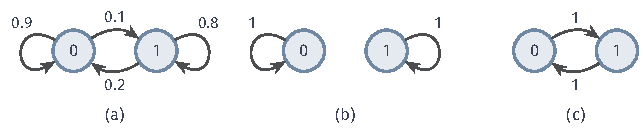
\includegraphics[width=109mm]{figures/07-probability/08-sampling-and-integration/tikz/mcerr-two-state/figure.pdf}
 \caption{两状态链的转移图，箭头上的数为转移概率。(a)$a=0.1$，$b=0.2$，不可约且非周期；(b)$a=b=0$，两个状态各自吸收，链可约；(c)$a=b=1$，不可约但周期为$2$。}
 \label{fig:mcerr-two-state}
\end{BookInlineFigure}

图~\ref{fig:mcerr-two-state}(b)与(c)是条件不成立的两种情形。可约链（$a=b=0$）就是上一节始终停在原地的例子，$\hat{I}_N=f(X^{(0)})$，既不趋于$I$，也没有正态极限。周期链（$a=b=1$）在$0,1$之间严格交替，从$\pi$出发时$\lambda=-1$，式~\eqref{eq:mcerr-two-state-lrv}给出$\sigma_{\mathrm{LR}}^{2}=0$：$N$为偶数时$\hat{I}_N$恰好等于$1/2$，误差比$N^{-1/2}$小得多，正态近似退化。从固定的状态$0$出发时，$X^{(t)}$的分布在两个单点之间来回切换，永远不趋于$\pi$，时间平均却仍然收敛。可见非周期性主要关系到边缘分布的收敛，不可约性关系到时间平均能否看到整个目标。

\paragraph{一般状态空间}
状态连续时，“以几何速度趋于目标”需要允许依赖初值的常数。若存在$r<1$与函数$M(x)$，对$\pi$几乎所有的$x$有$M(x)<\infty$，且
\begin{equation}
 d_{\mathrm{TV}}\bigl(K^{t}(x,\cdot),\pi\bigr)\leq M(x)\,r^{t},\qquad t=1,2,\dots ,
 \label{eq:mcerr-geometric-ergodic}
\end{equation}
就称链\term{几何遍历}（geometrically ergodic）。式中$t$步后的转移分布与目标之间的总变差按几何速度衰减，衰减的比例不依赖初值，起点越远只是常数$M(x)$越大。

链~\eqref{eq:mcerr-ar1}是几何遍历的。由式~\eqref{eq:mcerr-ar1-marginal}，$K^{t}(x,\cdot)$与$\pi$只差均值$\rho^{t}x$和方差$1-\rho^{2t}$。图~\ref{fig:mcerr-geo-ergodic}用数值积分算出$\rho=0.9$时的总变差：从$x=3$与$x=10$出发，曲线最终与$0.9^{t}$平行，起点越远曲线越高；从$x=0$出发，均值没有偏离，只剩方差的差别，衰减得更快，按$0.81^{t}$下降。

\begin{BookInlineFigure}
 \centering
 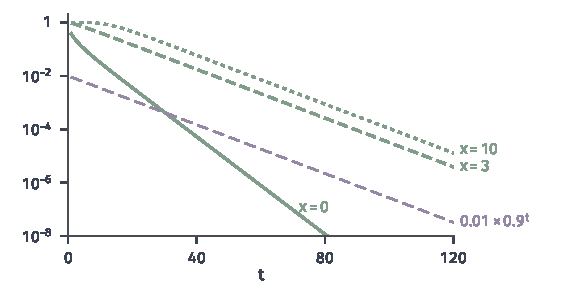
\includegraphics[width=96mm]{figures/07-probability/08-sampling-and-integration/matplotlib/mcerr-geo-ergodic/figure.pdf}
 \caption{链~\eqref{eq:mcerr-ar1}在$\rho=0.9$时，$t$步转移分布$\mathcal{N}(0.9^{t}x,1-0.81^{t})$与$\mathcal{N}(0,1)$的总变差（数值积分），绿色实线、虚线、点线分别为$x=0,3,10$；紫色虚线为参考斜率$0.01\times0.9^{t}$，纵轴为对数刻度。}
 \label{fig:mcerr-geo-ergodic}
\end{BookInlineFigure}

几何遍历配合比二阶稍强的矩条件，就足以给出正态极限。

\begin{theorem}[几何遍历链的中心极限定理]
\label{thm:mcerr-geo-clt}
设链以$\pi$为不变分布且几何遍历，$f$满足$\mathbb{E}_{\pi}\lvert f\rvert^{2+\delta}<\infty$，其中$\delta>0$。则平稳自协方差绝对可和，$\sigma_{\mathrm{LR}}^{2}<\infty$，并且链从$\pi$出发时
\begin{equation}
 \sqrt{N}\,\bigl(\hat{I}_N-I\bigr)\xrightarrow{\mathrm{d}}\mathcal{N}\bigl(0,\sigma_{\mathrm{LR}}^{2}\bigr) .
 \label{eq:mcerr-geo-clt}
\end{equation}
\end{theorem}

证明要估计相隔$k$步的两个函数值之间的依赖如何随$k$衰减，再用前面提到的鞅增量分解，篇幅较长，读者可查阅~\scite{math-meyn2009markov}。在卷九所讨论的常返条件下，结论对任意初始分布也成立。矩条件中的$\delta$一般不能取为零：对某些几何遍历的链，只满足$\mathbb{E}_{\pi}[f^{2}]<\infty$的$f$可以使$\sigma_{\mathrm{LR}}^{2}=\infty$，这类反例的构造较复杂。对链~\eqref{eq:mcerr-ar1}，$f(x)=x$或$x^{2}$的各阶矩都有限，定理适用，$f(x)=x$的极限方差就是$19$。

\paragraph{可和协方差不足以给出正态极限}
第~\ref{sec:mcerr-long-run}小节的方差极限只用了协方差绝对可和。下面的例子说明，仅有这一条不能推出正态极限。链的状态是一对$(W,Y)$。初始时$W$以各$1/2$的概率取$1$或$3$，此后永不改变；每一步$Y$重新抽取为$W\varepsilon$，其中$\varepsilon\sim\mathcal{N}(0,1)$与过去独立。转移核是
\[
 K\bigl((w,y),\cdot\bigr)=\delta_{w}\otimes\mathcal{N}(0,w^{2}) ,
\]
不变分布是“$W$各以$1/2$取$1,3$，给定$W$后$Y\sim\mathcal{N}(0,W^{2})$”。

取$f(w,y)=y$，$I=0$。平稳时
\[
 \gamma_0=\mathbb{E}[W^{2}]=5,\qquad \gamma_k=\mathbb{E}\bigl[W^{2}\varepsilon_0\varepsilon_k\bigr]=0\quad(k\geq1) ,
\]
自协方差除$\gamma_0$外全为零，绝对可和，长期方差$\sigma_{\mathrm{LR}}^{2}=5$，而且$N\operatorname{Var}(\hat{I}_N)$对每个$N$都等于$5$。可是
\[
 \sqrt{N}\,\hat{I}_N=W\cdot\frac{1}{\sqrt{N}}\sum_{t=1}^{N}\varepsilon_t ,
\]
后一个因子精确服从$\mathcal{N}(0,1)$且与$W$独立，所以$\sqrt{N}\hat{I}_N$对每个$N$都服从两个正态分布的等权混合，不是正态分布。它的四阶矩是$3\mathbb{E}[W^{4}]=123$，而方差为$5$的正态分布四阶矩是$75$。图~\ref{fig:mcerr-chain-clt}(b)中直方图中间更尖、两侧更厚，与$\mathcal{N}(0,5)$明显不同。原因是这条链可约：$W$一旦选定就再也不变，时间平均永远记得它。

\begin{BookInlineFigure}
 \centering
 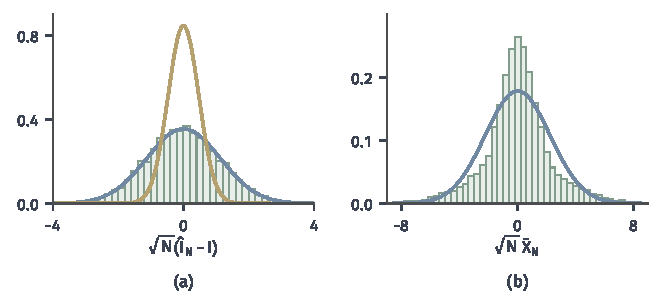
\includegraphics[width=112mm]{figures/07-probability/08-sampling-and-integration/matplotlib/mcerr-chain-clt/figure.pdf}
 \caption{链平均的极限分布。(a)两状态链$a=0.1$，$b=0.2$，从状态$0$出发，$N=2000$，$20000$条独立链（种子$3124$）的$\sqrt{N}(\hat{I}_N-1/3)$（绿色直方图），蓝线为$\mathcal{N}(0,34/27)$，黄线为误用单值方差的$\mathcal{N}(0,2/9)$；(b)可约链$(W,Y)$的$\sqrt{N}\hat{I}_N=WZ$的$20000$次抽样（绿色，种子$3125$），蓝线为$\mathcal{N}(0,5)$。}
 \label{fig:mcerr-chain-clt}
\end{BookInlineFigure}

\subsection{长期方差的估计}
\label{sec:mcerr-lrv-estimation}

即使中心极限定理成立，误差区间还需要$\sigma_{\mathrm{LR}}^{2}$的值。普通样本方差$S_N^{2}$估计的是$\gamma_0$，不是$\sigma_{\mathrm{LR}}^{2}$；用$S_N^{2}/N$作链平均的方差，在正相关时会把误差低估。下面两种估计都从同一条记录出发，分别从“分块”和“求和”两个方向逼近长期方差。

\paragraph{批均值}
由定理~\ref{thm:mcerr-long-run-limit}，长度为$b$的一段平稳记录，其平均的方差约为$\sigma_{\mathrm{LR}}^{2}/b$。若$b$远大于相关性的持续长度，相隔一段的两段平均几乎不相关。把记录切成$a$段，每段长$b$，$N=ab$，第$j$段的平均记为$\bar{Y}_j$。这$a$个段均值近似为方差$\sigma_{\mathrm{LR}}^{2}/b$的独立观测，于是它们的样本方差乘以$b$就估计了$\sigma_{\mathrm{LR}}^{2}$：
\begin{equation}
 \hat{\sigma}_{\mathrm{BM}}^{2}=\frac{b}{a-1}\sum_{j=1}^{a}\bigl(\bar{Y}_j-\hat{I}_N\bigr)^{2} .
 \label{eq:mcerr-batch-means}
\end{equation}
这种方法称为\term{批均值法}（batch means method）。$b=1$时每段只有一个值，式~\eqref{eq:mcerr-batch-means}退回普通样本方差$S_N^{2}$。

下面用一段短记录演示计算。两状态链（$a=0.1$，$b=0.2$）从不变分布出发运行$16$步（种子$3144$），$f$为状态$1$的示性函数，记录为
\[
 0,0,0,0,\ 0,0,1,0,\ 1,1,1,1,\ 1,0,0,0 .
\]
其中有六个$1$，$\hat{I}_{16}=6/16=0.375$。先算普通样本方差：六个值与平均相差$0.625$，十个值相差$-0.375$，
\[
 S_{16}^{2}=\frac{6\times0.625^{2}+10\times0.375^{2}}{15}=\frac{3.75}{15}=0.25 .
\]
再取段长$4$，分成四段，如图~\ref{fig:mcerr-batches}。段均值为
\[
 \bar{Y}_1=0,\quad \bar{Y}_2=0.25,\quad \bar{Y}_3=1,\quad \bar{Y}_4=0.25 .
\]
它们与$\hat{I}_{16}$的差的平方和为
\[
 0.375^{2}+0.125^{2}+0.625^{2}+0.125^{2}=0.5625 ,
\]
代入式~\eqref{eq:mcerr-batch-means}，
\[
 \hat{\sigma}_{\mathrm{BM}}^{2}=\frac{4}{3}\times0.5625=0.75 .
\]
两种估计给出的标准误差分别是
\[
 \sqrt{0.25/16}=0.125,\qquad \sqrt{0.75/16}=0.217 .
\]
真实的$\sigma_{\mathrm{LR}}^{2}=1.259$，平稳时的标准误差为$\sqrt{1.259/16}=0.281$。普通样本方差把它低估了一半以上；批均值的方向是对的，但只有四段，估计本身很粗糙。

\begin{BookInlineFigure}
 \centering
 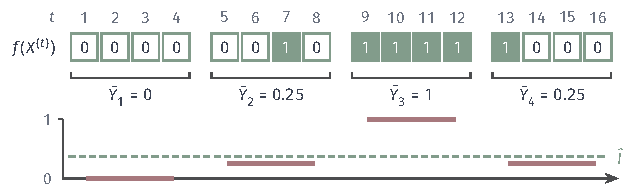
\includegraphics[width=107mm]{figures/07-probability/08-sampling-and-integration/tikz/mcerr-batches/figure.pdf}
 \caption{批均值的计算。上排为两状态链$16$步的函数值$f(X^{(t)})$（绿色方格为$1$），按长度$4$分成四段；下方红色横线为各段平均$\bar{Y}_j$，绿色虚线为总平均$\hat{I}=0.375$。段均值之间的离散程度反映了长期方差。}
 \label{fig:mcerr-batches}
\end{BookInlineFigure}

\paragraph{截断的自协方差和}
另一条路是直接按定义~\ref{def:mcerr-long-run}求和。由记录估计自协方差
\[
 \hat{\gamma}_k=\frac1N\sum_{t=1}^{N-k}\bigl(f(X^{(t)})-\hat{I}_N\bigr)\bigl(f(X^{(t+k)})-\hat{I}_N\bigr) ,
\]
再截断到$L$步：
\begin{equation}
 \hat{\sigma}_{L}^{2}=\hat{\gamma}_0+2\sum_{k=1}^{L}w_k\,\hat{\gamma}_k .
 \label{eq:mcerr-truncated-sum}
\end{equation}
权重$w_k=1$是直接截断；取$w_k=1-k/(L+1)$可以保证估计非负。不能对所有$k\leq N-1$求和：大$k$的$\hat{\gamma}_k$只由很少几对数据算出，噪声很大，全部加起来以后误差不随$N$缩小。

\paragraph{块长与截断的选择}
两种估计都面临同一个取舍。块长$b$或截断$L$太小，漏掉了尚未衰减的相关，估计偏低；太大，段数太少或加入太多噪声项，估计波动很大。图~\ref{fig:mcerr-lrv-estimates}在链~\eqref{eq:mcerr-ar1}（$\rho=0.9$）上用十条长度$2^{16}$的记录演示：$b=1$时批均值约为$\gamma_0=1$；$b=128$时十次的平均为$17.7$，仍偏低；$b=512$时平均为$18.7$，十次的标准差为$1.6$；$b=4096$时只剩$16$段，标准差增大到$7.9$。截断和的情形相同，$L$约为$60$时最稳定。

\begin{BookInlineFigure}
 \centering
 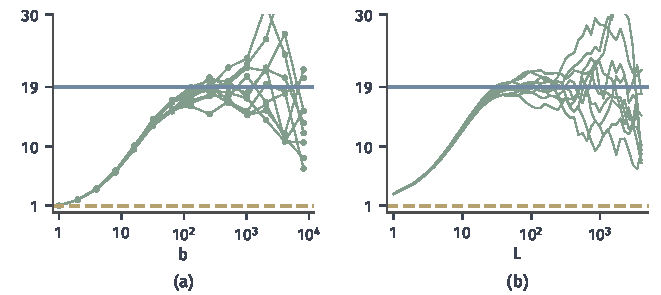
\includegraphics[width=112mm]{figures/07-probability/08-sampling-and-integration/matplotlib/mcerr-lrv-estimates/figure.pdf}
 \caption{长期方差的两种估计，链~\eqref{eq:mcerr-ar1}，$\rho=0.9$，$f(x)=x$，十条长度$N=2^{16}$的平稳记录（绿线，种子$3130$）。(a)批均值估计随块长$b$的变化；(b)直接截断的自协方差和随截断步数$L$的变化。蓝线为$\sigma_{\mathrm{LR}}^{2}=19$，黄色虚线为$\gamma_0=1$，横轴为对数刻度。}
 \label{fig:mcerr-lrv-estimates}
\end{BookInlineFigure}

要使估计一致，$b$与$a=N/b$都必须随$N$趋于无穷，例如$b$取$\sqrt{N}$的量级；截断和则要求$L\to\infty$且$L/N\to0$。此外还需要链以足够快的速度遍历，$f$满足比二阶更高的矩条件。证明需要把链的部分和与连续时间的随机路径作细致比较，超出本卷范围。

\paragraph{链平均的误差区间}
把三块拼起来：只有在链平均满足中心极限定理、$\sigma_{\mathrm{LR}}^{2}>0$且$\hat{\sigma}^{2}$是一致估计时，由Slutsky定理，
\[
 \frac{\sqrt{N}\,(\hat{I}_N-I)}{\hat{\sigma}}\xrightarrow{\mathrm{d}}\mathcal{N}(0,1) ,
\]
从而区间$\hat{I}_N\pm z\hat{\sigma}/\sqrt{N}$的覆盖概率趋于$1-\alpha$。这里的$\hat{\sigma}^{2}$是$\hat{\sigma}_{\mathrm{BM}}^{2}$或$\hat{\sigma}_{L}^{2}$，不能用$S_N^{2}$代替。三个条件中任何一个不成立，区间都没有保证：可约链没有正态极限，周期链可能$\sigma_{\mathrm{LR}}^{2}=0$，块长不当则方差估计不一致。

\subsection{运行诊断的边界}
\label{sec:mcerr-diagnostics}

上面的条件涉及链的遍历性质，通常无法从记录中验证。实践中用一些运行诊断来发现问题，它们各有用处，也各有盲区。

\paragraph{一个双峰目标}
取$\pi$为$\mathcal{N}(-5,1)$与$\mathcal{N}(5,1)$的等权混合，$f(x)=x$，$I=0$。用第~\ref{chap:sample-generation}章的随机游走Metropolis算法：从当前状态$x$提出候选$y=x+\eta$，$\eta\sim\mathcal{N}(0,1)$，以概率$\min\{1,\tilde{p}(y)/\tilde{p}(x)\}$接受，否则留在$x$，其中$\tilde{p}$是$\pi$的密度。这条链以$\pi$为不变分布，并且候选可以到达任何位置，理论上能在两个峰之间往返。问题在于两峰之间密度很低：$x=0$处的密度只有峰值的$2\mathrm{e}^{-12.5}\approx7\times10^{-6}$倍，每一步只能移动一个单位左右，穿越低谷需要连续多次接受向下的移动，这几乎不会发生。

图~\ref{fig:mcerr-bimodal-traces}(a)从$-7,-3,3,7$出发运行四条链，每条$5000$步（种子$3131$），接受率约为$0.70$。四条链没有一次穿过$0$：两条留在左峰，平均为$-5.00$与$-5.01$；两条留在右峰，平均为$5.05$与$4.95$。链间的分歧明白地暴露了问题。把四条链合在一起，平均为$-0.004$，碰巧接近$0$，但这只是因为初值恰好两边各两个；若三条从左边出发，合并平均就在$-2.5$附近。两峰各占多少质量，这些记录完全没有测量到。

图(b)把四条链都放在左侧，从$-7,-6,-4,-3$出发（种子$3132$）。四条链的平均分别为$-4.98,-4.98,-5.03,-4.94$，彼此一致；轨迹看起来平稳，运行平均早已停住，每条链的估计有效样本量也不小。所有诊断都通过了，答案却是$-4.98$而不是$0$。

\begin{BookInlineFigure}
 \centering
 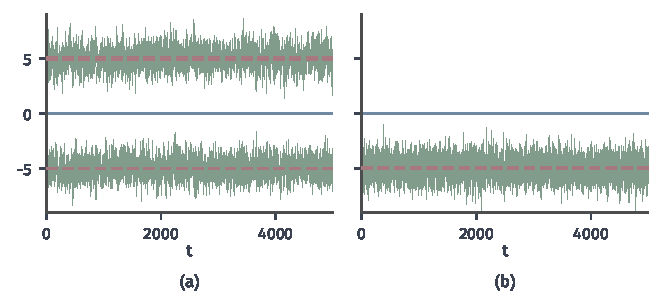
\includegraphics[width=112mm]{figures/07-probability/08-sampling-and-integration/matplotlib/mcerr-bimodal-traces/figure.pdf}
 \caption{双峰目标$\frac12\mathcal{N}(-5,1)+\frac12\mathcal{N}(5,1)$上的随机游走Metropolis链，每条$5000$步。绿线为轨迹，红色虚线为每条链的平均，蓝线为$I=0$。(a)从$-7,-3,3,7$出发（种子$3131$）；(b)从$-7,-6,-4,-3$出发（种子$3132$）。}
 \label{fig:mcerr-bimodal-traces}
\end{BookInlineFigure}

\paragraph{各种诊断能看到什么}
表~\ref{tab:mcerr-diagnostics}总结了常用的几种诊断。比较多次运行时，常同时看链间平均的差异与链内的波动：若链间差异远大于链内波动所能解释的范围，说明各链还没有忘掉初值或停在不同区域。\term{轨迹图}（trace plot）即状态随步数的曲线，\term{运行均值}（running mean）即前$t$步平均随$t$的曲线。

\begin{BookInlineTable}
 \centering
 \caption{运行诊断的作用与盲区}
 \label{tab:mcerr-diagnostics}
 \begin{tabular}{p{25mm}p{36mm}p{36mm}}
  \toprule
  诊断 & 能发现 & 不能发现 \\
  \midrule
  不同初值的多次运行 & 初值影响，停在不同区域 & 所有初值都未到达的区域 \\
  轨迹图 & 趋势，缓慢移动，停滞 & 从未访问的区域 \\
  运行均值 & 尚未稳定的漂移 & 稳定在错误值上 \\
  估计的有效样本量 & 强相关，方差估计不稳 & 只在局部区域混合良好 \\
  \bottomrule
 \end{tabular}
\end{BookInlineTable}

这些诊断共同的盲区是：有限的记录只能告诉我们链去过哪里，不能告诉我们还有哪里没去。双峰例子里，记录中没有任何信息提示右边还有一半质量；第~\ref{sec:mcerr-asymptotic-interval}小节的稀有大贡献是同一现象在独立样本中的版本。所以诊断的结论只能是否定性的：诊断失败说明有问题，诊断通过不说明没有问题。误差区间所需的遍历性与矩条件，需要从目标与转移的结构分析得到，例如知道目标的峰在哪里，或者证明转移满足几何遍历；运行诊断不能替代这些理论条件。


\section{整组随机化的误差}
\label{sec:mcerr-replication}

有些采样方法一次产生一组彼此相关的点：每个点单独看都服从目标分布，但点与点之间被有意安排，使整组覆盖得更均匀。第~\ref{chap:variance-reduction}章的拉丁超立方采样与随机化准Monte Carlo都属于这一类。这样的组内平均无偏，方差却不能用独立公式计算，同一组点的样本方差也不反映它。办法是把整组当作一个观测单位，独立地重复整个构造。

\paragraph{整体平移的网格}
用一个最简单的构造说明。目标仍是$I=\int_0^1\mathrm{e}^{u}\,\mathrm{d}u$。取$n$个等距点$a_i=(i-1)/n$，$i=1,\dots,n$，再取一个$\Delta\sim\operatorname{Unif}(0,1)$，把所有点一起平移并按模$1$回绕：
\[
 U_i=(a_i+\Delta)\bmod1 .
\]
对固定的$a\in[0,1)$与$s\in[0,1]$，使$(a+\Delta)\bmod1\leq s$的$\Delta$构成$[0,1)$中总长度为$s$的一个或两个区间，所以每个$U_i$都服从$\operatorname{Unif}(0,1)$。由第~\ref{sec:mcerr-estimator}节，组平均
\[
 Q=\frac1n\sum_{i=1}^{n}f(U_i)
\]
是$I$的无偏估计。但这些点完全不独立：知道一个点，就知道了整组。

$n=4$时，组平均只依赖$\Delta'=\Delta\bmod\tfrac14$：四个点就是$\Delta'+j/4$，$j=0,1,2,3$。对$f(u)=\mathrm{e}^{u}$，等比求和给出
\begin{equation}
 Q=\frac{\mathrm{e}^{\Delta'}}{4}\sum_{j=0}^{3}\mathrm{e}^{j/4}=c\,\mathrm{e}^{\Delta'},\qquad c=\frac{\mathrm{e}-1}{4(\mathrm{e}^{1/4}-1)}=1.5124 .
 \label{eq:mcerr-shift-q}
\end{equation}
四个点均匀地分布在$[0,1)$上，相互弥补，$\operatorname{Var}(Q)=0.01536$；同样四个独立均匀点的平均，方差是$\sigma_f^{2}/4=0.0605$，大了约四倍。组内的依赖正是精度提高的来源，也正是它使独立公式失效。

\subsection{组间方差}
\label{sec:mcerr-between-var}

固定每组点数$n$，用独立的随机数重复同一个随机化规则$R$次，得到组估计$Q_1,\dots,Q_R$。它们独立同分布，每一个都是一次完整构造的结果。

\begin{theorem}[组间方差估计]
\label{thm:mcerr-between-var}
设$Q_1,\dots,Q_R$独立同分布，$\mathbb{E}[Q_1]=I$，$\mathbb{E}[Q_1^{2}]<\infty$，$R\geq2$。令
\begin{equation}
 \bar{Q}=\frac1R\sum_{r=1}^{R}Q_r,\qquad s_Q^{2}=\frac{1}{R-1}\sum_{r=1}^{R}\bigl(Q_r-\bar{Q}\bigr)^{2} .
 \label{eq:mcerr-between}
\end{equation}
则$\mathbb{E}[\bar{Q}]=I$，并且
\begin{equation}
 \operatorname{Var}(\bar{Q})=\frac{\operatorname{Var}(Q_1)}{R},\qquad \mathbb{E}\Bigl[\frac{s_Q^{2}}{R}\Bigr]=\operatorname{Var}(\bar{Q}) .
 \label{eq:mcerr-between-unbiased}
\end{equation}
\end{theorem}

\begin{proof}
前两条是独立同分布变量平均的期望与方差，与定理~\ref{thm:mcerr-iid-bound}的证明相同。记$v=\operatorname{Var}(Q_1)$。把每一项写成$Q_r-\bar{Q}=(Q_r-I)-(\bar{Q}-I)$，展开平方和，并利用$\sum_r(Q_r-I)=R(\bar{Q}-I)$，
\[
 \sum_{r=1}^{R}\bigl(Q_r-\bar{Q}\bigr)^{2}=\sum_{r=1}^{R}(Q_r-I)^{2}-R\,(\bar{Q}-I)^{2} .
\]
取期望，第一项为$Rv$，第二项为$R\cdot v/R=v$，所以
\[
 \mathbb{E}\Bigl[\sum_{r=1}^{R}\bigl(Q_r-\bar{Q}\bigr)^{2}\Bigr]=(R-1)\,v .
\]
除以$R-1$得$\mathbb{E}[s_Q^{2}]=v$，再除以$R$即得结论。
\end{proof}

定理只用到组与组之间的独立，对组内点的依赖没有任何要求。这正是需要的分工：组内怎样安排由设计决定，误差由组间的波动来度量。反过来，把$nR$个点混在一起求样本方差再除以$nR$，相当于假装这些点彼此独立，没有依据。

\paragraph{四组的计算}
取$n=4$，$R=4$，四次平移为
\[
 \Delta_1=0.37,\quad \Delta_2=0.81,\quad \Delta_3=0.19,\quad \Delta_4=0.64 ,
\]
如图~\ref{fig:mcerr-group-shift}(a)。按模$\tfrac14$约化，$\Delta'$依次为$0.12,0.06,0.19,0.14$。代入式~\eqref{eq:mcerr-shift-q}，
\[
 Q_1=1.7053,\quad Q_2=1.6060,\quad Q_3=1.8289,\quad Q_4=1.7397 .
\]
总平均为$\bar{Q}=1.7200$，与$I=1.7183$相差$0.0017$。各组与总平均的差是$-0.0147,-0.1140,0.1089,0.0198$，由式~\eqref{eq:mcerr-between}，
\[
 s_Q^{2}=0.008491,\qquad \frac{s_Q^{2}}{R}=0.002123,\qquad \sqrt{s_Q^{2}/R}=0.0461 .
\]
真实的$\operatorname{Var}(\bar{Q})=0.01536/4=0.00384$，标准差为$0.0620$；只有四组时，估计值$0.0461$偏小，但这是随机波动，不是系统偏差。

若把$16$个函数值当作独立样本，它们的样本方差为$0.2483$，除以$16$得$0.01552$，标准误差$0.1246$，是真实值的两倍。它实际上估计的是$16$个独立点的方差$\sigma_f^{2}/16$，完全没有反映网格带来的改进。这里组内点相互弥补，独立公式高估了误差；若组内点彼此相似，例如一段链记录，独立公式就会低估误差。两个方向的错误都来自同一个原因：用组内的离散程度代替了组间的波动。

图~\ref{fig:mcerr-group-shift}(b)把整个实验（每次$R=4$组）重复$5000$次。正确估计$s_Q^{2}/R$的平均为$0.00382$，与真实值$0.00384$一致，但分布很宽，因为每次只有四个组估计；混合估计集中在$0.0159$附近，稳定地错了四倍。

\begin{BookInlineFigure}
 \centering
 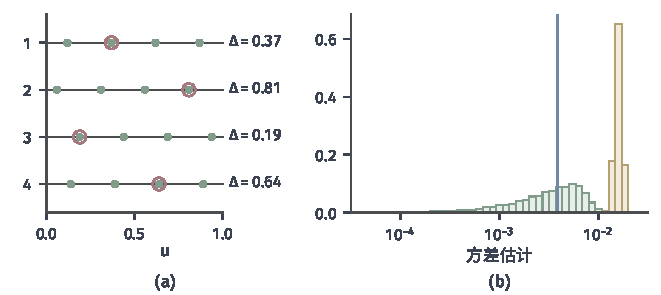
\includegraphics[width=112mm]{figures/07-probability/08-sampling-and-integration/matplotlib/mcerr-group-shift/figure.pdf}
 \caption{整体平移网格估计$\int_0^1\mathrm{e}^{u}\,\mathrm{d}u$，每组$n=4$点。(a)四组点（绿点），红圈为各组的平移量$\Delta_r$；(b)整个实验（$R=4$）重复$5000$次（种子$3133$）：绿色为$s_Q^{2}/R$的分布，黄色为把$16$个值当作独立样本的估计，蓝线为真实的$\operatorname{Var}(\bar{Q})=0.00384$，横轴为对数刻度。}
 \label{fig:mcerr-group-shift}
\end{BookInlineFigure}

\subsection{渐近误差区间}
\label{sec:mcerr-replication-interval}

组估计$Q_1,\dots,Q_R$是独立同分布的观测，第~\ref{sec:mcerr-asymptotic-interval}小节的结论可以原样搬过来，只是把“样本”换成“整组”，把样本数$N$换成重复数$R$。若$n$固定，$0<\operatorname{Var}(Q_1)<\infty$，则由定理~\ref{thm:mcerr-iid-clt}，$R\to\infty$时
\begin{equation}
 \frac{\sqrt{R}\,(\bar{Q}-I)}{s_Q}\xrightarrow{\mathrm{d}}\mathcal{N}(0,1) ,
 \label{eq:mcerr-replication-clt}
\end{equation}
区间$\bar{Q}\pm z\,s_Q/\sqrt{R}$的覆盖概率趋于$1-\alpha$。

上面的四组给出区间
\[
 1.7200\pm1.96\times0.0461=[1.6297,\,1.8103] ,
\]
包含$I$。但$R=4$离“$R\to\infty$”很远。由式~\eqref{eq:mcerr-shift-q}，$Q$是$\Delta'$的指数函数，取值在一个有界区间内，并不服从正态分布。用$20$万次重复实验（种子$3134$）估计，这个区间的实际覆盖概率在$R=4$时为$0.840$，$R=10$时为$0.917$，$R=30$时为$0.939$，$R=100$时为$0.947$。

对少量重复，常见的做法是把$z$换成自由度为$R-1$的t分布分位数，$R=4$时为$3.182$。若各组估计恰好服从正态分布，这能给出精确的覆盖概率；但组估计一般不是正态的，本例中这样做的覆盖概率是$0.929$，仍低于$0.95$。所以少量整组重复只能给出近似的误差范围，不提供有限样本下的精确覆盖保证。

这一节的结论可以概括为两条。第一，组内点边缘分布正确只保证无偏，不意味着它们彼此独立，组内的样本方差不衡量估计的误差。第二，独立重复的整组是误差估计的基本单位，误差区间的可靠程度由重复数$R$决定，而不是由总点数$nR$决定。第~\ref{chap:variance-reduction}章设计组内结构以减小$\operatorname{Var}(Q)$时，都按这里的方式估计误差。


\section{本章小结}
\label{sec:mcerr-summary}

Monte Carlo估计$\hat{I}_N$的误差总是分成偏差与随机波动两部分。偏差只取决于各个样本的分布是否等于$\pi$，与样本是否独立无关；波动取决于样本之间的依赖与被积函数的矩。两部分必须分别评价：增加样本数只压低波动，从不消除偏差，而偏差又无法从输出本身读出。

\paragraph{各种来源的误差}
表~\ref{tab:mcerr-summary}按样本来源列出本章的主要结论。

\begin{BookInlineTable}
 \centering
 \caption{不同样本来源下的误差}
 \label{tab:mcerr-summary}
 \begin{tabular}{lll}
  \toprule
  样本来源 & 偏差 & 波动的尺度 \\
  \midrule
  独立、精确 & 零 & $\sigma_f^{2}/N$，需二阶矩 \\
  独立、近似$\tilde{\pi}$ & $\mathbb{E}_{\tilde{\pi}}f-\mathbb{E}_{\pi}f$，不随$N$变 & $\operatorname{Var}_{\tilde{\pi}}(f)/N$ \\
  链、从一般初值出发 & 由边缘分布的收敛速度控制 & 同下 \\
  链、平稳 & 零 & 渐近为$\sigma_{\mathrm{LR}}^{2}/N$ \\
  整组随机化 & 零（各点边缘正确时） & $\operatorname{Var}(Q)/R$ \\
  \bottomrule
 \end{tabular}
\end{BookInlineTable}

\paragraph{保证的类型}
独立样本有两类保证。Chebyshev界对每个$N$成立，只需二阶矩，但偏松；渐近误差区间更紧，但只在$N\to\infty$时给出名义覆盖，稀有的大贡献可以使所需的$N$大到无法从样本中察觉。只有一阶矩时大数律仍成立，但误差可以按慢于$N^{-1/2}$的速度缩小。

近似生成的偏差由总变差控制，前提是被积函数有界；无界时还要控制两种分布的尾部或矩。近似转移先要确认存在不变分布，再估计它与$\pi$的差别。

链平均的初值偏差需要边缘分布趋于$\pi$的速度估计，舍弃初始一段只有在这种估计下才有依据，对无界函数还需要一致可积。平稳链平均的方差由自协方差决定，长期方差是它的极限，有效样本量是它的换算，三者都依赖被积函数。链平均的误差区间同时需要中心极限定理、正的长期方差和一致的长期方差估计；运行诊断只能发现问题，不能证明链已遍历目标。

一次产生一组相关点的方法，以独立重复的整组为观测单位，用组间的样本方差估计误差，可靠程度由重复数决定。

\paragraph{与后续各章的关系}
第~\ref{chap:variance-reduction}章改变抽样分布、估计公式或抽样机制来减小波动，每一种改变都会改变估计量的分布，因而都要按本章的方式重新检查偏差、矩条件和样本之间的依赖。第~\ref{chap:expectation-gradient-estimation}章估计期望的导数时，近似采样带来的偏差同样不能靠样本数消除。第~\ref{chap:sampling-budget-method-selection}章在给定预算下分配样本，所比较的正是本章给出的偏差与方差。

